\subsection*{Общая характеристика работы}

\newcommand{\actuality}{\underline{\textbf{Актуальность темы.}}}
\newcommand{\aim}{\underline{\textbf{Целью}}}
\newcommand{\tasks}{\underline{\textbf{задачи}}}
\newcommand{\defpositions}{\underline{\textbf{Основные положения, выносимые на~защиту:}}}
\newcommand{\novelty}{\underline{\textbf{Научная новизна:}}}
\newcommand{\influence}{\underline{\textbf{Научная и практическая значимость}}}
\newcommand{\reliability}{\underline{\textbf{Достоверность}}}
\newcommand{\probation}{\underline{\textbf{Апробация работы.}}}
\newcommand{\contribution}{\underline{\textbf{Личный вклад.}}}
\newcommand{\publications}{\underline{\textbf{Публикации.}}}



{\actuality} В настоящее время известно большое количество исследований магнетизма и сверхпроводимости соединений с атомами переходных металлов\cite{Slocombe_2015}.
Неорганические соединения, включающие в себя атомы с 3d\textsuperscript{9} электронной оболочкой и обладающие несимметричной поверхностью Ферми, такие как  керамические соединения купратов, тонкопленочные структуры  и монокристаллы с атомами интерметаллидов, представляют интерес для исследований и обладают практической ценностью как функциональные материалы.

Одним из актуальных исследований является работа \cite{Blandy_2018}, в которой экспериментально показано возникновение антиферромагнитного упорядочения в слоистой структуре Sr\textsubscript{2}CuO\textsubscript{2}Cu\textsubscript{2}S\textsubscript{2} на атомах меди Cu\textsuperscript{+} и Cu\textsuperscript{2+}.
Так, например, в работе, посвященной сверхпроводящим купратам\cite{Comin_2015}, отмечается высокая вероятность возникновения спин-флуктуационного механизма, который приводит к искажению поверхности Ферми и возникновению d\textsubscript{x\textsubscript{2}-y\textsubscript{2}}-симметрии параметра порядка вблизи атомов меди.
Наблюдаемые искажения приводят к возникновению переменной валентности на атомах меди и обусловлены особенностями кристаллической структуры: переходный металл находится в слоях между полиэдрами разной конфигурации, а образованные полиэдрами пустоты заполняются стабилизирующими структуру катионами.
Таким образом, создаются структурные комбинации, которые приводят к возникновению сложной электронной структуры.


Другими перспективными для исследования неорганическими материалами, в которых наблюдается переменная валентность на атомах одного сорта, являются соединения солей из группы тетраэдрита-теннантита.
В основе этих соединений лежит лавесовский полиэдр: усеченный тетраэдр (Рис.~\ref{img:figure1}).
Полиэдр сформирован 6 атомами меди, которые располагаются  в центре рёбер не усеченного тетраэдра.
Сформированный лавесовский полиэдр окружен тетраэдрическими комплексами, направленными в одну сторону.
  В такой структуре тетраэдритов и теннантитов, ввиду ян-тейллоровского искажения,   наблюдается сдвиг атомов меди из идеального положения, который приводит к  перекрытию электронных орбиталей атомов меди и формирует особенную электронную структуру.
Высокая чувствительность электронной структуры к расстоянию между атомами меди и чувствительность к окружению лавесовского полиэдра  делает соединения из группы тетраэдрита--теннантита  интересными для исследований и прикладных применений.

В современной литературе эти соединения рассматриваются как функциональные материалы для термоэлектриков ввиду их низкой теплопроводности, вызванной наличием изолированных комплексов в структуре.
Некоторые соединения из этой группы обладают магнитными свойствами, которые возникают благодаря сложным ионно--ковалентным связям. В некоторых работах отмечается возможное магнитное упорядочение в соединениях теннантита и тетраэдрита.
Также преимущественно сульфосоли являются индикаторами золотосодержащих руд, потребность в которых высока.

В данной работе представлено исследование влияния изовалентного замещения в соединениях Cu\textsubscript{12}As\textsubscript{4}S\textsubscript{13}, Cu\textsubscript{12}Sb\textsubscript{4}S\textsubscript{13}, Cu\textsubscript{3}AsSe\textsubscript{3} и Cu\textsubscript{3}SbSe\textsubscript{3} на транспортные и магнитные свойства этих соединений.
Также в работе приведено рентгеноструктурное исследование соединения  Cu\textsubscript{12}As\textsubscript{4}S\textsubscript{13} в диапазоне температур от 85 до 293~К.  Помимо полученных фундаментальных результатов данная работа вносит вклад в развитие современного материаловедения и дополняет существующие представления о механизмах формирования физических свойств.

 \aim\ данного исследования является определение положения атомов меди в синтетическом теннантите
 Cu\textsubscript{12}As\textsubscript{4}S\textsubscript{13}, изучение на его примере особенностей формирования лавесовского полиэдра и влияния изовалентного замещения на магнитные и транспортные свойства соединений из группы тетраэдрита--теннантита на примере соединений  Cu\textsubscript{12}As\textsubscript{4}S\textsubscript{13}, Cu\textsubscript{12}Sb\textsubscript{4}S\textsubscript{13}, Cu\textsubscript{3}AsSe\textsubscript{3} и Cu\textsubscript{3}SbSe\textsubscript{3}.

Для~достижения поставленной цели необходимо было решить следующие основные {\tasks}:
\begin{enumerate}
  \item Исследование положения атомов меди методами монокристальной	 рентгеновской дифрактометрии, высокоразрешающей микроскопии и комбинационного рассеяния света в монокристаллическом образце синтетического теннантита Cu\textsubscript{12}As\textsubscript{4}S\textsubscript{13} в диапазоне температур от 85 до 300~К.
  \item Измерение зависимостей теплоёмкости образцов Cu\textsubscript{12}As\textsubscript{4}S\textsubscript{13} и Cu\textsubscript{3}AsSe\textsubscript{3} и магнитной восприимчивости  образцов Cu\textsubscript{12}As\textsubscript{4}S\textsubscript{13}, Cu\textsubscript{12}Sb\textsubscript{4}S\textsubscript{13}, Cu\textsubscript{3}AsSe\textsubscript{3} и Cu\textsubscript{3}SbSe\textsubscript{3} в диапазонах температур от 2  до 350~К методами сканирующей дифференциальной калориметрии и магнитометрии.

\end{enumerate}

\defpositions
\begin{enumerate}
\item Показано, что синтетический теннантит Сu\textsubscript{12}As\textsubscript{4}S\textsubscript{13} обладает неэквивалентным  окружением атомов меди в позициях Cu21 и Cu2 и в элементарной ячейке содержится 12 атомов меди.
\item Неэквивалентные позиции атомов меди Cu21 и Cu2 в синтетическом теннантите приводят к разным химическим потенциалам структуры, которые, возможно, являются движущей силой для возникновения позиции Cu21.
\item В синтетическом теннантите Сu\textsubscript{12}As\textsubscript{4}S\textsubscript{13} обнаружен фазовый переход второго рода при температуре 124~К методами рентгеноструктурного анализа, сканирующей дифференциальной калориметрии и магнитометрии.
\item В соединениях синтетических теннантита Сu\textsubscript{12}As\textsubscript{4}S\textsubscript{13} и мгриита Cu\textsubscript{3}AsSe\textsubscript{3} экспериментально выявлены низкоэнергетических фононных моды, наличие которых обусловлено  ассиметричной связью As(CuS\textsubscript{3})As.
\item Показано, что изовалентное замещение Cu--(As,Sb)--S приводит к изменению локального окружения атомов меди и приводит к понижению температуры Нееля с $\approx$124 К до $\approx$84 К.

\end{enumerate}

\novelty
\begin{enumerate}
\item Уточнена структурная формула синтетического теннантита Сu\textsubscript{12}As\textsubscript{4}S\textsubscript{13}.
\item По результатам рентгеноструктурного анализа, анализа спектра комбинационного рассеяния света и квантовомеханических расчётов синтетического теннантита Сu\textsubscript{12}As\textsubscript{4}S\textsubscript{13} обнаружено влияние ассиметричной связи As(CuS\textsubscript{3})As на размягчение фононных мод в структуре синтетического теннантита Сu\textsubscript{12}As\textsubscript{4}S\textsubscript{13}.
\item В соединении  синтетического теннантита Сu\textsubscript{12}As\textsubscript{4}S\textsubscript{13} обнаружен фазовый переход второго рода
 при 124~К методами рентгеноструктурного анализа, сканирующей дифференциальной калориметрии и магнитометрии.
\item Методами сканирующей дифференциальной калориметрии и спектроскопии комбинационного рассеяния света обнаружены низкоэнергетические фононные моды для соединений из группы тетраэдритов-теннантитов в диапазоне от 5 до 40~мэВ.
\item Обнаружено влияние изовалентного замещения в Cu--(As,Sb)--S и  Cu--(As,Sb)--Se на значения температурных диапазонов  особых магнитных состояний.
\end{enumerate}

\influence\ заключается в уникальных научных данных, которые выявляют связь наблюдаемых физических характеристик с особенностями кристаллической структуры.
Результаты структурных и спектроскопических исследований показывают причины возникновения низкой теплопроводности и позволяют осознанно производить поиск новых функциональных соединений с характерными тетраэдритами в структуре. Результаты квантовомеханических расчётов показывают причины возникновения переменной валентности в структуре синтетического теннантита и делают соединения группы тетраэдрита--теннантита интересными с точки зрения изучения магнитных свойств.
Температурные зависимости магнитной восприимчивости изовалентных аналогов синтетического теннантита и температурные исследования структуры синтетического теннантита могут быть использованы для планирования дальнейших исследований магнитных фазовых превращений в соединениях группы тетраэдрита--теннантита.

\reliability\ полученных результатов обеспечивается комплексными
исследованиями материалов  методами рентгеновской монокристальной дифрактометрии, электронной просвечивающей микроскопии, калориметрии, исследованием намагниченности и транспортных свойств и применением современного оборудования
сертифицированного в соответствии с российскими и международными стандартами.
Достоверность и высокое качество полученных результатов
подтверждается публикациями материалов работы в рецензируемых научных журналах из перечня ВАК, а также докладами на российских и международных
конференциях.
Часть полученных результатов воспроизводит результаты, ранее полученные другими авторами.

\probation\
Основные результаты работы докладывались~на российских и международных конференциях:
\begin{itemize}
\item  XXV Российская молодежная научная конференция, посвященная 95"~летию основания Уральского университета, <<Проблемы теоретической и экспериментальной химии>>, 22"--~24 апреля 2015, г. Екатеринбург;
\item Вторая Всероссийская молодежная научно-техническая конференция с международным участием <<Инновации в материаловедении>>, 1"--~4 июня 2015, г. Москва;
\item Международная Конференция, посвященная 80"~летию чл."~кор. РАН И.К. Камилова, <<Фазовые переходы, критические и нелинейные явления в конденсированных средах>>,  20"--~28 августа 2015, г. Челябинск;
\item ХII Российская ежегодная конференция молодых научных сотрудников и аспирантов <<Физико-химия и технология неорганических материалов>>, 13"--~16 октября 2015, г. Москва;
\item III Всероссийская научная молодежная конференция
<<Актуальные проблемы нано- и микроэлектроники>>, с 30 октября по 4 декабря 2015, г.~Уфа;
\item III Международная молодёжная научная конференция: Физика. Технологии. Инновации ФТИ"--~2016, 16"--~20 мая 2016, г. Екатеринбург;
\item Международная конференция молодых ученых, работающих в области углеродных материалов, с 30 мая по 1 июня 2017, г. Троицк, г. Москва;
\item Cедьмая международная конференция <<Кристаллофизика и деформационное поведение перспективных материалов>>, посвященная памяти профессора С.С. Горелика, c 2"--~5 октября 2017, г. Москва.
\end{itemize}


%и самостоятельно сформулировал \textcolor{red}{научную проблему --- проблему чего}
\contribution\ В диссертации представлены результаты, полученные лично соискателем, либо при его личном участии. Автор диссертации принимал непосредственное участие в выборе используемых методик. В работах по теме диссертации, выполненных с соавторами, автору диссертации принадлежит постановка целей и задач, анализ, обработка и обобщение полученных результатов экспериментов. Автором использованы алгоритмы обработки данных, на основе которых получены два свидетельства о государственной регистрации программ для электронно-вычислительных машин №~2018664257 от 14.11.2018 и №~2018664530 от 19.11.2018.

%\publications\ Основные результаты по теме диссертации изложены в ХХ печатных изданиях~\cite{Sokolov,Gaidaenko,Lermontov,Management},
%Х из которых изданы в журналах, рекомендованных ВАК~\cite{Sokolov,Gaidaenko},
%ХХ --- в тезисах докладов~\cite{Lermontov,Management}.

\ifthenelse{\equal{\thebibliosel}{0}}{% Встроенная реализация с загрузкой файла через движок bibtex8
    \publications\ Основные результаты по теме диссертации изложены в XX печатных изданиях,
    X из которых изданы в журналах, рекомендованных ВАК,
    X "--- в тезисах докладов.%
}{% Реализация пакетом biblatex через движок biber
%Сделана отдельная секция, чтобы не отображались в списке цитированных материалов
    \begin{refsection}%
        \printbibliography[heading=countauthornotvak, env=countauthornotvak, keyword=biblioauthornotvak, section=1]%
        \printbibliography[heading=countauthorvak, env=countauthorvak, keyword=biblioauthorvak, section=1]%
        \printbibliography[heading=countauthorconf, env=countauthorconf, keyword=biblioauthorconf, section=1]%
        \printbibliography[heading=countauthor, env=countauthor, keyword=biblioauthor, section=1]%
        \publications\ Опубликовано 16 работ в печатных изданиях, в том числе 8 работ в журналах, рекомендованных ВАК. Основные результаты по теме диссертации изложены в 12 %\arabic{citeauthor}
 печатных изданиях\nocite{vakbibl9,vakbibl8,vakbibl2,vakbibl1,vakbibl7,vakbibl5,vakbibl6,vakbibl4}, %,,conf8,conf7,conf6,conf5,conf4,conf3,conf2,conf1
       4 %\arabic{citeauthorvak}
из которых изданы в журналах, рекомендованных ВАК,
%\nocite{vakbibl2,vakbibl1,vakbibl7}, %,vakbibl5,vakbibl4,\arabic{citeauthorconf}
8 "--- в тезисах докладов.
%\nocite{conf8,conf7,conf6,conf5,conf4,conf3,conf2,conf1}.
    \end{refsection}
}
%При использовании пакета \verb!biblatex! для автоматического подсчёта
%количества публикаций автора по теме диссертации, необходимо
%их здесь перечислить с использованием команды \verb!\nocite!.
 % Характеристика работы по структуре во введении и в автореферате не отличается (ГОСТ Р 7.0.11, пункты 5.3.1 и 9.2.1), потому её загружаем из одного и того же внешнего файла, предварительно задав форму выделения некоторым параметрам

%Диссертационная работа была выполнена при поддержке грантов ...

%\underline{\textbf{Объем и структура работы.}} Диссертация состоит из~введения, четырех глав, заключения и~приложения. Полный объем диссертации \textbf{ХХХ}~страниц текста с~\textbf{ХХ}~рисунками и~5~таблицами. Список литературы содержит \textbf{ХХX}~наименование.

%\newpage
\subsection*{Содержание работы}
Во \underline{\textbf{введении}} обосновывается актуальность исследований, проводимых в рамках данной диссертационной работы, приводится обзор научной литературы по изучаемой теме, формулируется цель, ставятся задачи работы. Также сформулированы научная новизна и практическая значимость представляемой работы.

В \underline{\textbf{первой главе}} проведен обзор литературных данных по структурным, транспортным и магнитным свойствам соединений из группы тетраэдрита-теннантита. Проанализированы особенности строения теннантита и тетраэдрита. Особое внимание уделено особенностям влияния локального окружения меди на формирование тепловых и магнитных свойств.

В современной литературе рассмотрены основные механизмы и условия образования структуры трёхкомпонентных халькогенидов меди (ТХМ).
В опубликованных данных\cite{Pfitzner1998a} отмечается, что соединения обладают изоморфизмом и необходимо ответственно подходить к синтезу соединений: точно соблюдать режимы синтеза и стехиометрическое соотношение.

Физические свойства ТХМ связываются с особенностями их структуры. Структура ТХМ представляют собой тетраэдрические комплексы  CuVI\textsubscript{4}, где VI = S, Se, ориентированные в пространстве в одну сторону (Рис. \ref{img:figure1}а).
Такое упорядочение тетраэдрических комплексов создает пустоты таким образом, что между  комплексами образуются лавесовские полиэдры (в форме усеченных тетраэдров), которые изображены на рисунке~\ref{img:figure1}б). В~полученных усеченных тэтраэдрах помещается по шесть атомов меди (Рис.~\ref{img:figure1}в), к каждому из которых относится три атома серы\cite{Makovicky_2006}.
Термоэлектрические и магнитные свойства в данных соединениях связываются с особенностью распределения меди в лавесовских полиэдрах  и разориентировкой тетраэдрических комплексов в структуре. Так, например, аномально низкая теплопроводность связывается с ангармоническими тепловыми колебаниями в~позиции атомов меди\cite{Mishra2017} и ассиметричными связями\cite{Lai_2015}. Такие ассиметричные связи приводят к появлению мягкой моды, которая квазилокализована и обладает низкой фононной частотой и большой амплитудой. Подобные связи объясняют природу низкой теплопроводности в тетраэдритах и высоких значений термоэлектрической эффективности\cite{Lu2013}. В литературе отмечается\cite{Lai_2015}, что энергия таких мод составляет $\approx$~5 мэВ. А изменение электронной структуры и, как следствие, изменение магнитных свойств связываются с трансформацией комплексов  Cu\textsubscript{6}(S,Se)\textsubscript{12} при понижении температуры\cite{Gainov2008}. В то же время, опубликованные данные о фазовых превращениях различны и в них не прослеживается общих трендов.

\begin{figure}[ht]
  \begin{minipage}[ht]{0.3\linewidth}\centering
    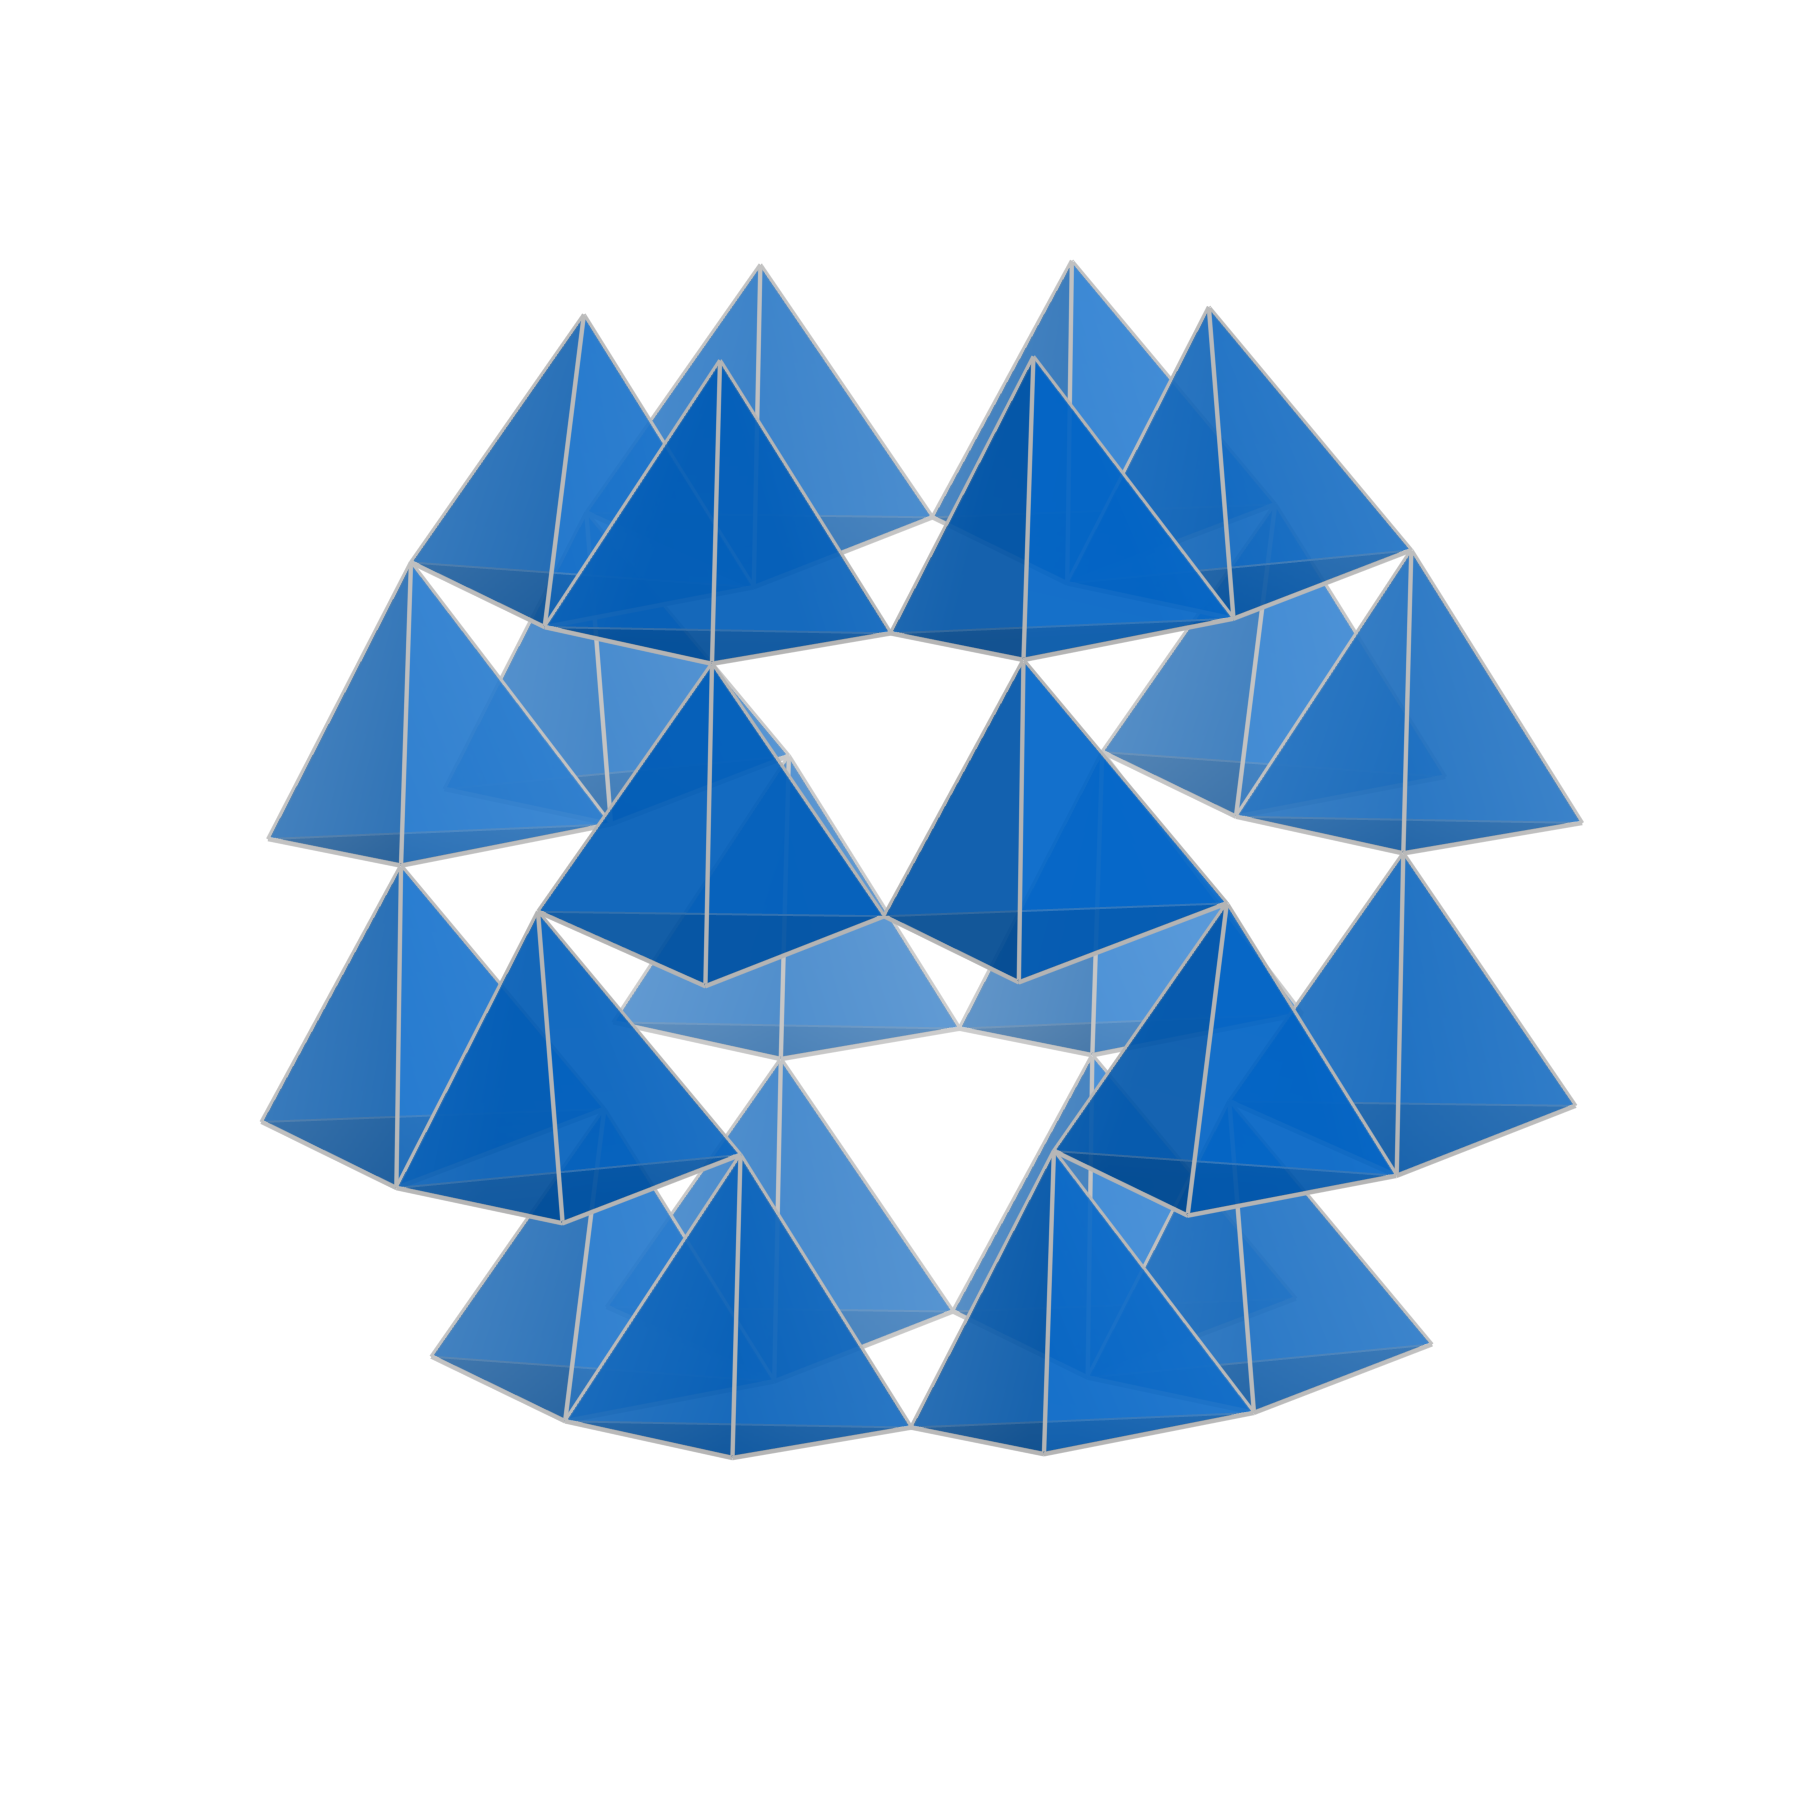
\includegraphics[width=0.9\linewidth]{1_cu12as4s13_crys_st_a} \\ а)
  \end{minipage}
  \hfill
  \begin{minipage}[ht]{0.3\linewidth}\centering
    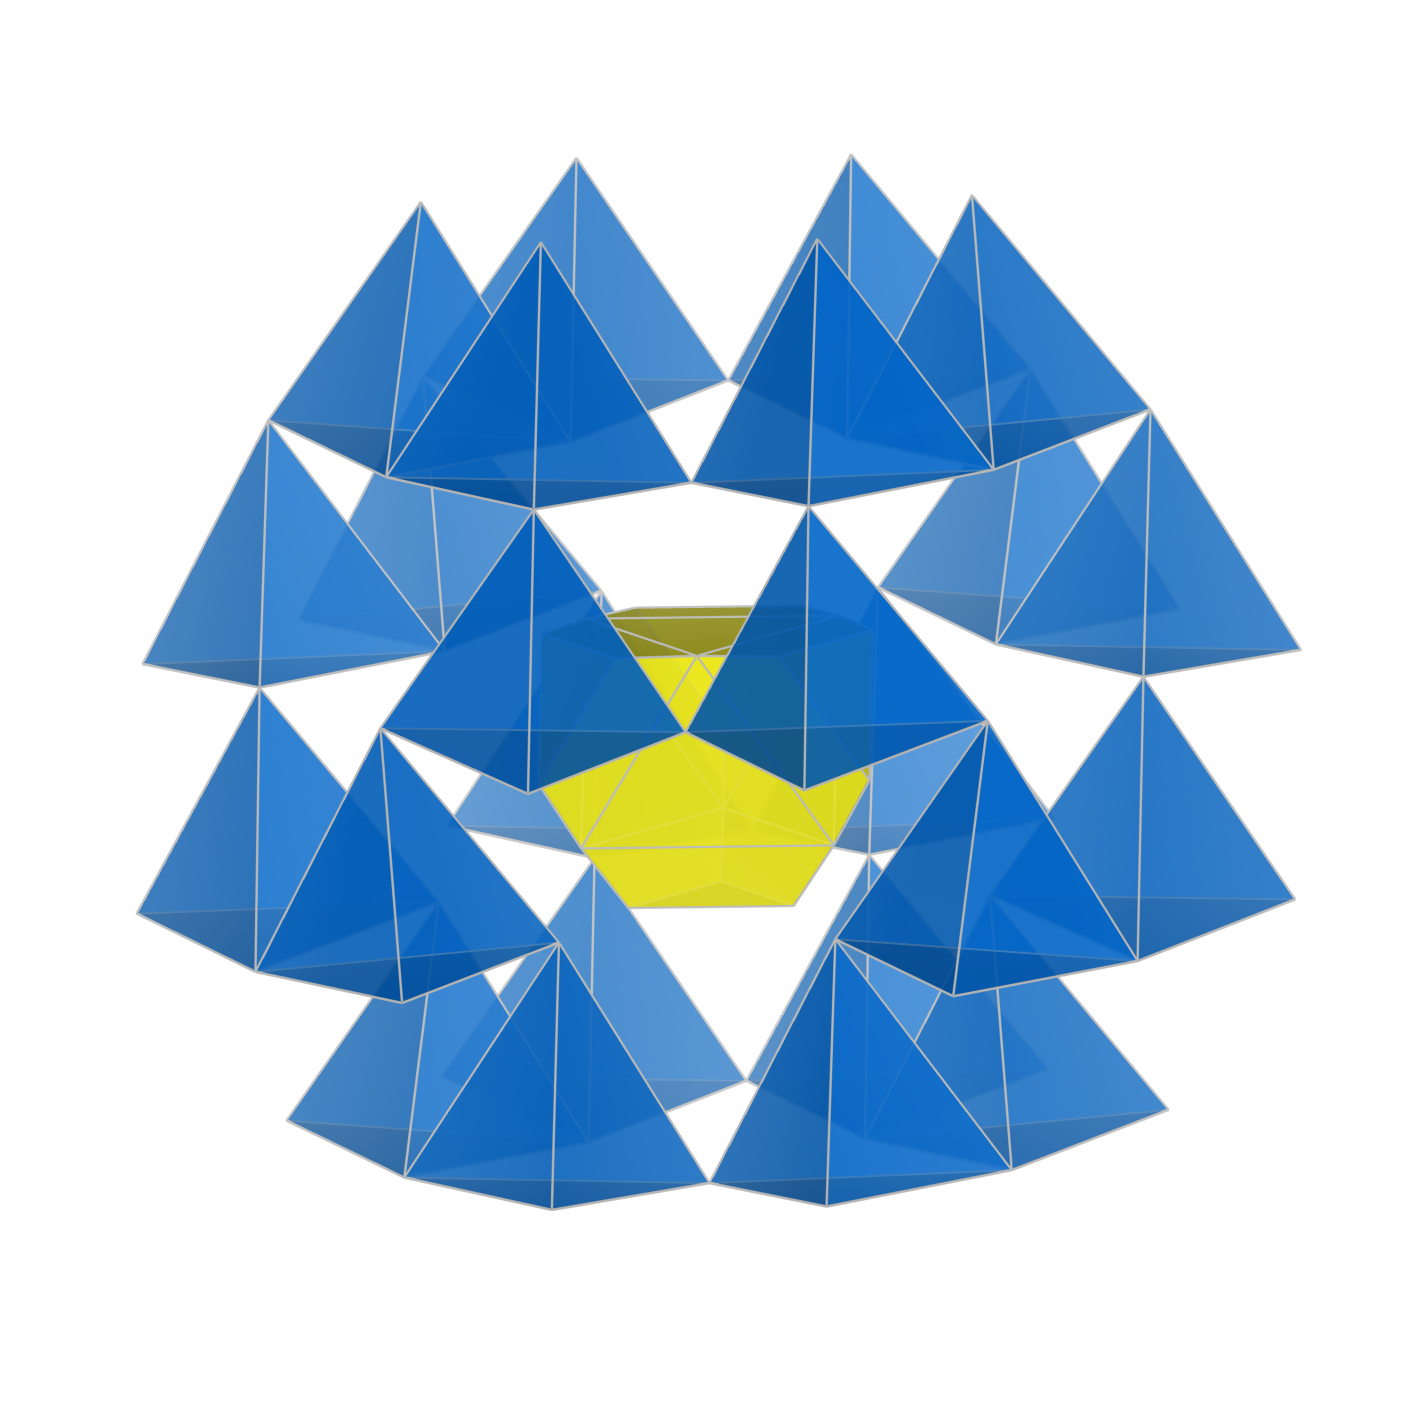
\includegraphics[width=0.9\linewidth]{2_cu12as4s13_crys_st_b} \\ б)
  \end{minipage}
\hfill
 \begin{minipage}[ht]{0.3\linewidth}\centering
    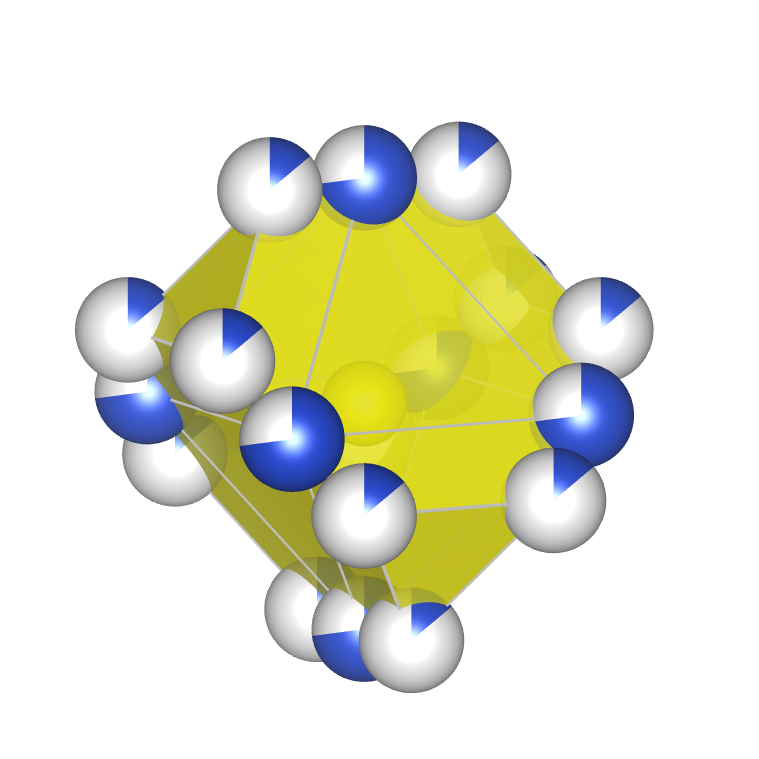
\includegraphics[width=0.9\linewidth]{3_cu12as4s13_crys_st_c} \\ в)
  \end{minipage}
      \caption[Кристаллическая структура халькогенида на примере синтетического теннантита Cu\textsubscript{12}As\textsubscript{4}S\textsubscript{13}]{Кристаллическая структура халькогенида на примере синтетического теннантита Cu\textsubscript{12}As\textsubscript{4}S\textsubscript{13}}
    \label{img:figure1}
\end{figure}

Также в главе дан обзор основных литературных данных о физических свойствах халькогенидов, в частности,  магнитных и транспортных\cite{bab_81}.
По данным \cite{bab_1982,DiBenedetto2002, Bernardini2000,Gainov2008} в структуре возможно возникновение антиферромагнитного упорядочения при понижении температуры. В работах \cite{Lu2013,Lara-Curzio2014,Tablero2014,Lu2016,Nasonova2016} проведены исследования стабильности полиморфных фаз и проанализированы возможности использования соединений в качестве функциональных материалов для термоэлектрических устройств.



Во \underline{\textbf{второй главе}} описаны методики исследования и методы синтеза соединений для систем Cu--As--S, Cu--Sb--S, Cu--As--Se и Cu--Sb--Se в~стехиометрическом соотношении.
А именно: методы порошковой и монокристальной дифрактометрии, измерения и моделирования теплоёмкости, просвечивающей электронной микроскопии, комбинационного рассеяния света и измерения магнитной восприимчивости. Также описаны условия проведения квантовомеханических расчётов.

Соединения Cu\textsubscript{12}V\textsubscript{4}VI\textsubscript{13}, где V = As, Sb и VI = S, Se синтезированы в~кварцевых ампулах с инертной средой. В~качестве исходных материалов использованы реактивы высокой чистоты не ниже марки <<особо чистый>>. Исходная шихта составлена в соотношении 3Cu:1V:3VI
(избыток по~сере или селену составлял не~более 3"--~5~\%). Точность определения температуры в~рабочей камере печи соответствовала 0,5~К при 600~К и 1~К при 1100~К (для контроля температуры использовалась термопара платина/платина "--- 10~\% родий). Синтез проведен в~четыре этапа. Первый~"--- медленное нагревание в~печи (10"--~15~часов) до~температуры, превышающей температуру плавления легколетучего компонента (серы или селена) на~10"--~30~К; второй~"--- поддержание данной температуры 20"--~30~часов. После этого увеличение температуры до~полного плавления образовавшегося в~ампуле вещества в течении 40"--~50~ч. и поддержание этой температуры постоянной 20"--~30 ч. Последний этап"--- понижение температуры до 2/3 от температуры плавления и отжиг соединения 30"--~40~ч. Образец Cu\textsubscript{12}As\textsubscript{4}S\textsubscript{13} после спекания дополнительно был подвергнут направленной перекристаллизации в~двухзонной печи по~методу Стокбаргера"--~Бриджмена. Часть образцов дополнительно была отожженна при~температуре 673 и 773~К в~течении 24~часов.

Исследования образцов проведены методами рентгенофазового и энергодисперсионного анализов.
Рентгенофазовый анализ осуществлен методом порошка на образцах, которые  получены дроблением исходных спеченных образцов до гомогенного состояния в ступке. Дифрактограммы  обрабатывались в~программном комплексе Jade~6 с использованием реферативной базы pdf2. Полученные образцы аттестованы на порошковом дифрактометре D8 Advance (Bruker, Германия) на Cu K$\alpha$ излучении. Три соединения из синтезированных  идентифицированы в кубической сингонии, одно --- в~тетрагональной cингонии.

Прецизионное исследование структуры монокристалла теннантита проведено на четырехкружном автоматическом дифрактометре Xcalibur c 2d детектором  CCD~EOS~S2 и с~системой охлаждения Cobra Plus при температурах 85, 115, 180, 250 и 293~K.
В работе исследовались сколы от монокристаллического образца с линейными размерами от 100 до 300~мкм.
Температурные эксперименты проведены с использованием характеристического Mo K\textsubscript{$\alpha$} изучения с длиной волны 0.71073~$\angstrom$. Дополнительно было проведено исследование структуры образца сферической формы синтетического теннантита при комнатной температуре.

Изображения атомных структур получены на электронном микроскопе FEI Titan 80--300 в режиме HAADF-STEM  при ускоряющем напряжении 300 кВ.
HAADF режим дает контраст по атомному номеру (зависимость Z\textsuperscript{2}).
Образец приготовлен с помощью системы фокусированного ионного пучка (FIB) на двухлучевом сканирующем микроскопе "--- FEI Helios 600.
Изображения получены при комнатной температуре на ламельке толщиной менее 100~нм и плоскости синтетического теннантита (011) Cu\textsubscript{12}As\textsubscript{4}S\textsubscript{13}.
Обработка изображений произведена в программном обеспечении atomap\cite{Nord2017}. С помощью программного обеспечения было проведено определение колонок атомов меди и их эллиптичности. Дополнительно был учтен дрейф и получены изображения, показывающие величину эллиптичности для рядов атомов меди в плоскости (011).

Теплоёмкость измерена при помощи измерительного комплекса PPMS (Quantum Design,
США) в диапазоне температур от 2 до 350 К. Измерения проводились методом релаксации теплового импульса\cite{Hwang_1997}. Измерительный комплекс представляет собой автономный комплекс с гелиевым криостатом замкнутого цикла. Расчётная кривая теплоёмкости получена вычислением функции Дебая с тремя дополнительными осцилляторами Эйнштейна. Выбор характеристических температур осцилляторов Эйнштейна описан в тексте диссертации. Добавление осцилляторов Эйнштейна рассматривается в описании экспериментальных данных и обуславливается смягчением фононных мод в соединениях.

Квантовомеханические вычисления проводились в рамках теории функционала плотности с использованием программы VASP (Vienna Ab initio Simulation Package) \cite{Kresse1993,Kresse1994,Kresse1996}, основанной на методе присоединённых плоских волн. Равновесная атомная геометрия зоны Бриллюэна была разбита  на 7~k"~точек с помощью метода Монкхоста--Пака (Monkhorst--Pack) \cite{Monkhorst_1976}. Величина энергии обрезания в расчёте равнялась 300~эВ. Оптимизация атомной структуры проводилась до тех пор, пока межатомные силы не становились меньше 0.005~эВ/${\angstrom}$.

Спектры комбинационного рассеяния получены на спектрометре TRIAX-552, оборудованном охлаждаемым детектором Peltier TE CCD SPEC 10 (Princeton Instruments).
Была использована решетка 600 штрихов на мм и 50-кратная линза Mitutoyo M Plan Apo SL50 (числовая апертура 0.42).
Для возбуждения спектров комбинационного рассеяния применен аргон-ионный лазер с длиной волны 514.5~нм Spectra-Physics Stabilite 2017 с выходной мощностью от 0.3 до 1~мВт на образце. Калибровка проведена с использованием линии спектра комбинационного рассеяния света 520.5~см\textsuperscript{-1} полированной кремниевой пластины и/или линий спектра комбинационного рассеяния неона.
Для получения спектра комбинационного рассеяния вблизи возбуждающей линии в оптической схеме были использованы 3  брэгговских фильтра.

Магнитные свойства образцов измерены с
помощью магнитоизмерительного комплекса
MPMS--XL7~EC (Quantum Design, США) с первичным преобразователем на основе СКВИДа в~диапазоне температур от 2 до 350 К и в постоянных магнитных полях напряженностью до 70 кЭ. Шаг измерения в диапазоне от $-$5 до 5~кЭ составлял 0.1~Э, при больших полях "--- 1~Э.

В \underline{\textbf{третьей главе}} представлены результаты исследования монокристаллического образца синтетического теннантита Cu\textsubscript{12}As\textsubscript{4}S\textsubscript{13} методами монокристальной дифрактометрии в диапазоне температур от 85 до 293~К, просвечивающей микроскопии монокристаллического образца в плоскости (011) и моделирования структур теннантита с разным расположением атомов в лавесовском полиэдре методом первопринципных расчётов.



Исследование монокристаллического образца  Cu\textsubscript{12}As\textsubscript{4}S\textsubscript{13} проведено при температурах 85, 115, 180, 250 и 293~К. Образцы получены сколом от монокристаллического образца с линейными размерами от 100 до 300~мкм.  Результаты дифракционных экспериментов при разных температурах представлены в таблице~\ref{xray1}. С понижением температуры объем элементарной ячейки ожидаемо уменьшается и возрастает значение R-фактора, a  заселенность позиции Cu2 (pис.~\ref{img:figure1}в) возрастает и  наблюдается аномальное изменение значения коэффициента атомарного смещения для позиции S2 (pис.~\ref{img:figure1}в), которое показывает наличие фазового перехода второго рода в диапазоне от 115 до 180 К.



\begin{landscape}
\begin{table} [htbp]
\centering
\caption{Сводная таблица данных рентгеноструктурных исследований для синтетического теннантита Cu\textsubscript{12}As\textsubscript{4}S\textsubscript{13} при температурах 85, 115, 180, 250 и 293~К}%
	\label{xray1}% label всегда желательно идти после caption
    \renewcommand{\arraystretch}{1.5}
	\begin{tabular}{@{}@{\extracolsep{20pt}}llllll@{}}
 \toprule     %%% верхняя линейка
T, K                       & 85          & 115         & 180         & 250         & 293         \\
   \midrule
a, $\angstrom$                       & 10.1439(2)  & 10.1446(2)  & 10.1463(2)  & 10.1523(2)  & 10.1572(2)  \\ \hline
V, $\angstrom^3$                      & 1043.79(4)      & 1044.01(4)      & 1044.54(4)      & 1046.39(4)      & 1047.91(4)      \\ \hline
Группа симметрии                     &\multicolumn{5}{c}{ I–43m  }                                         \\ \hline
Длина волны, ($\angstrom$) & \multicolumn{5}{c}{Mo K\textsubscript{$\alpha$}, 0.71069 } \\ \hline
Дифрактометр             & \multicolumn{5}{c}{Xcalibur}                                       \\ \hline
Коррекция абсорбции      & \multicolumn{5}{c}{аналитическая(по форме кристалла)} \\ \hline
$\theta_{max}$,\textsuperscript{ $\circ$ }                 &  \multicolumn{5}{c}{42.08 } \\ \hline
R\textsubscript{int}                       & 0.052       & 0.054       & 0.049       & 0.050       & 0.049       \\ \hline
N\textsubscript{ref} , регистрированный           & 11028       & 11029       & 11036       & 11010       & 11026       \\ \hline
I $\geq \sigma$(I)                  & 693         & 691         & 686         & 677         & 667         \\ \hline
N\textsubscript{paf}                       & 36          & 42          & 47          & 47          & 44          \\ \hline
GOF                        & 1.06        & 1.15        & 1.03        & 1.01        & 1.00        \\ \hline
R/R\textsubscript{w}                     & 0.034/0.052 & 0.037/0.056 & 0.031/0.045 & 0.032/0.045 & 0.029/0.038 \\ \hline
$\pm\Delta\rho   $                     & +2.9/–1.8   & +3.5/–1.7   & +2.3/–1.1   & +1.8/–1.1   & +1.7/–1.2   \\ \hline
R\textsubscript{MEM}                     & 0.017/0.021 & 0.016/0.021 & 0.018/0.022 & 0.018/0.022 & 0.019/0.021\\ \hline
 \bottomrule
\end{tabular}
\end{table}
\end{landscape}


Анализ изображения структуры показывает наличие распределенной электронной плотности в форме эллипса у некоторых рядов и косвенно подтверждает наличие сдвинутых атомов меди в структуре теннантита. На рисунке \ref{img:figure5}в) представлены атомарные ряды меди, которые имеют форму эллипса, с учётом дрейфа для плоскости (011) синтетического теннантита Cu\textsubscript{12}As\textsubscript{4}S\textsubscript{13}.


\begin{figure}[ht]
  \begin{minipage}[ht]{0.3\linewidth}\centering
    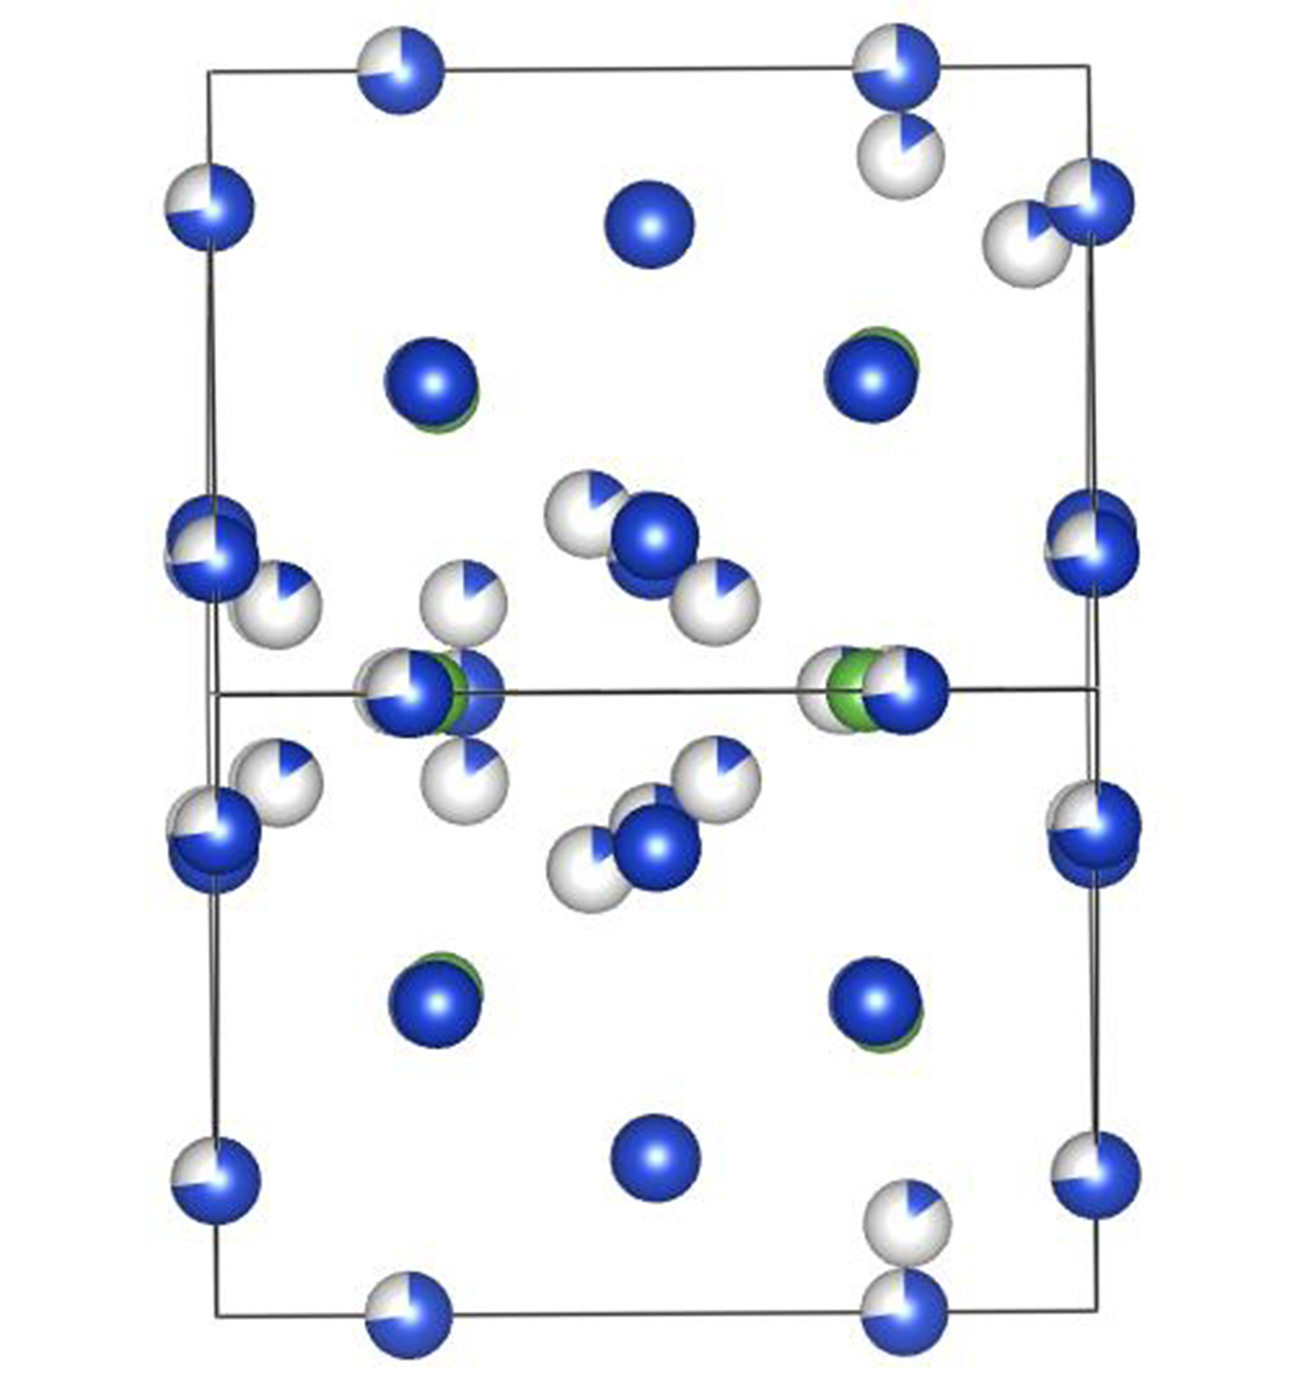
\includegraphics[width=0.9\linewidth]{mic_cu12as4s13_110_a} \\ а)
  \end{minipage}
  \hfill
  \begin{minipage}[ht]{0.3\linewidth}\centering
    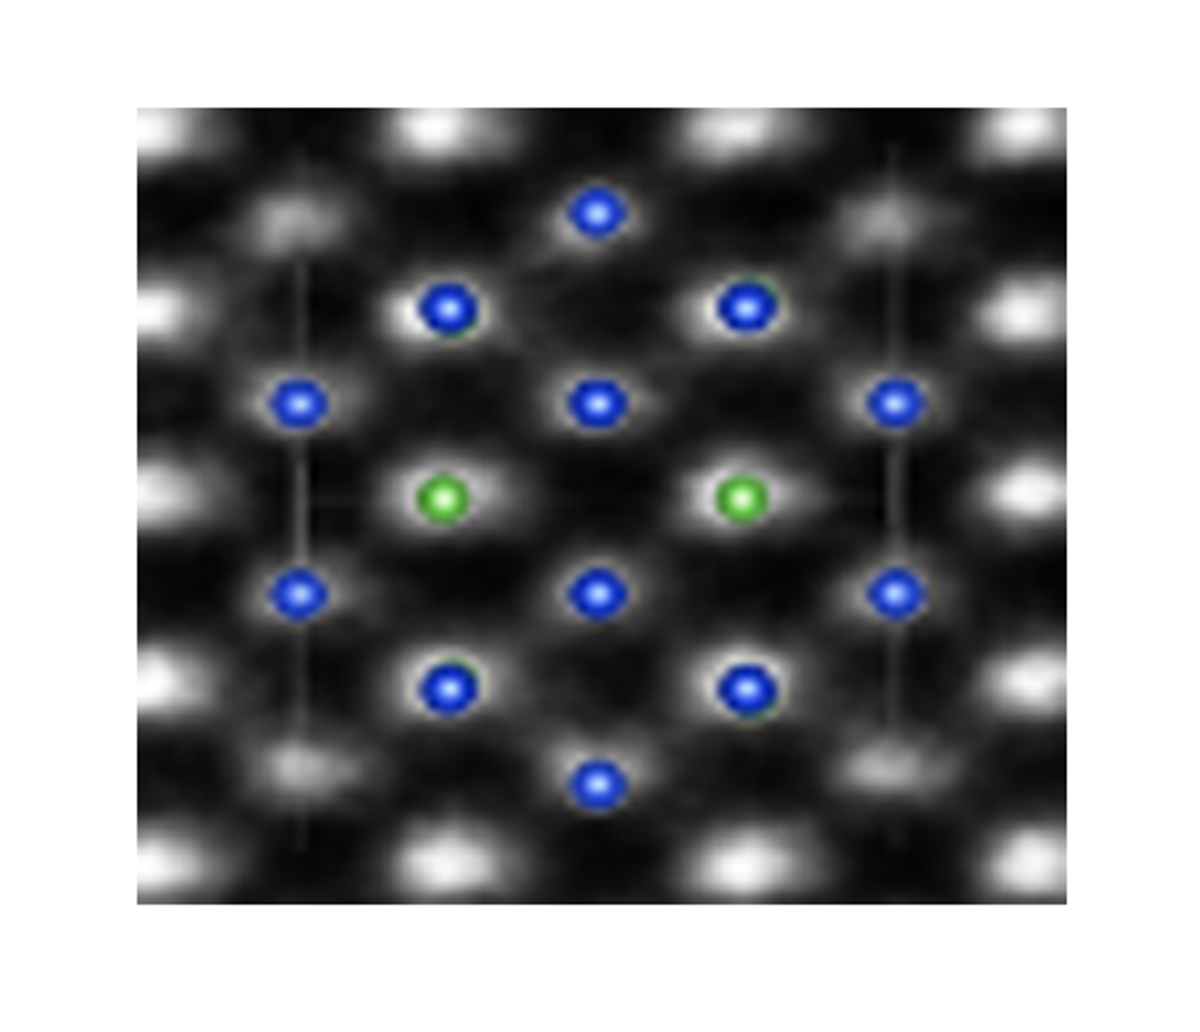
\includegraphics[width=0.9\linewidth]{mic_cu12as4s13_110_b} \\ б)
  \end{minipage}
  \hfill
  \begin{minipage}[ht]{0.3\linewidth}\centering
    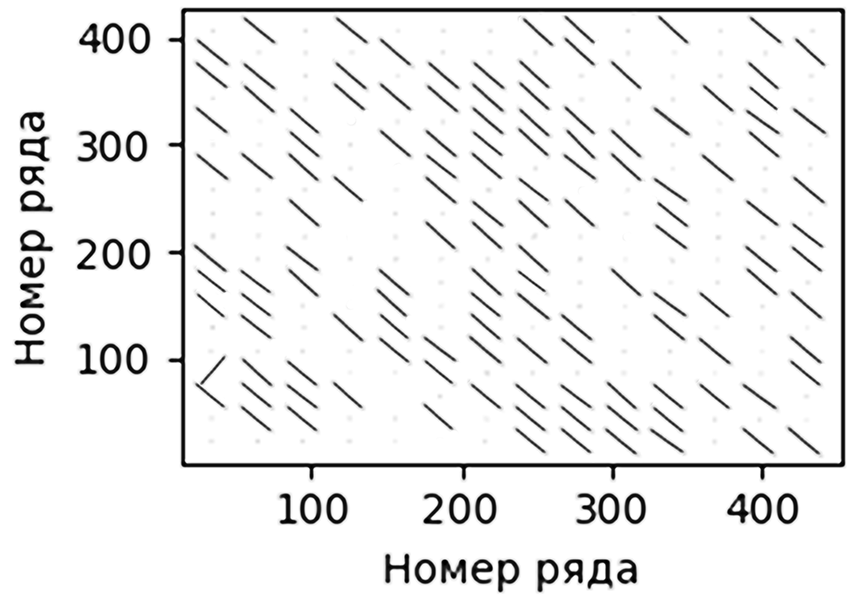
\includegraphics[width=0.9\linewidth]{mic_cupper_raw} \\ в)
  \end{minipage}
      \caption[Изображение расположения атомных рядов (синим обозначен атом меди, зеленым --- мышьяка) для синтетического теннантита Cu\textsubscript{12}As\textsubscript{4}S\textsubscript{13} в плоскости (011) (а), совмещенное изображение экспериментального изображения и атомарных рядов для синтетического теннантита Cu\textsubscript{12}As\textsubscript{4}S\textsubscript{13} в плоскости (011) (б),  изображение  рядов для атомов меди, в которых электронная плотность имеет форму эллипса и полученная после анализа атомарного изображения эллиптичность для рядов меди синтетического теннантита Cu\textsubscript{12}As\textsubscript{4}S\textsubscript{13} (в)]{Изображение расположения атомных рядов (синим обозначен атом меди, зеленым --- мышьяка) для синтетического теннантита Cu\textsubscript{12}As\textsubscript{4}S\textsubscript{13} в плоскости (011) (а), совмещенное изображение экспериментального изображения и атомарных рядов для синтетического теннантита Cu\textsubscript{12}As\textsubscript{4}S\textsubscript{13} в плоскости (011) (б),  изображение  рядов для атомов меди, в которых электронная плотность имеет форму эллипса и полученная после анализа атомарного изображения эллиптичность для рядов меди синтетического теннантита Cu\textsubscript{12}As\textsubscript{4}S\textsubscript{13} (в)}
    \label{img:figure5}
\end{figure}


Для исследования наиболее выгодного положения атомов меди были рассчитаны энергии 20 структур с разным положением атомов меди.
Структуры разделены на две группы: первая --- в лавесовском полиэдре сдвинуты 6 атомов меди (структуры с 1 по 10), вторая --- сдвинуты 3 атома меди в лавесовском полиэдре (структуры с 10 по 19).
На рисунке \ref{img:th} представлен график со значениями энергий элементарных ячеек для рассчитанных структур. Красной пунктирной линией обозначена энергия исходной структуры.
Экспериментальные структуры, полученные после анализа рентгеноструктурных данных  экспериментов при разных температурах, были рассчитаны с учетом ферромагнитного (ФМ), антиферромагнитного (АФМ), парамагнитного (ПМ) и диамагнитного состояний в структурах. 
Антиферромагнитное упорядочение в экспериментальной структуре при 85~К энергетически более выгодно, чем ферро-, пара- или диамагнитное состояния. При этом для 293~К ФМ, АФМ, ПМ конфигурации имеют одинаковую до (4 знака) энергию, что указывает на их одинаковую вероятность.

\begin{figure}[ht]
  \begin{minipage}[ht]{0.9\linewidth}\centering
    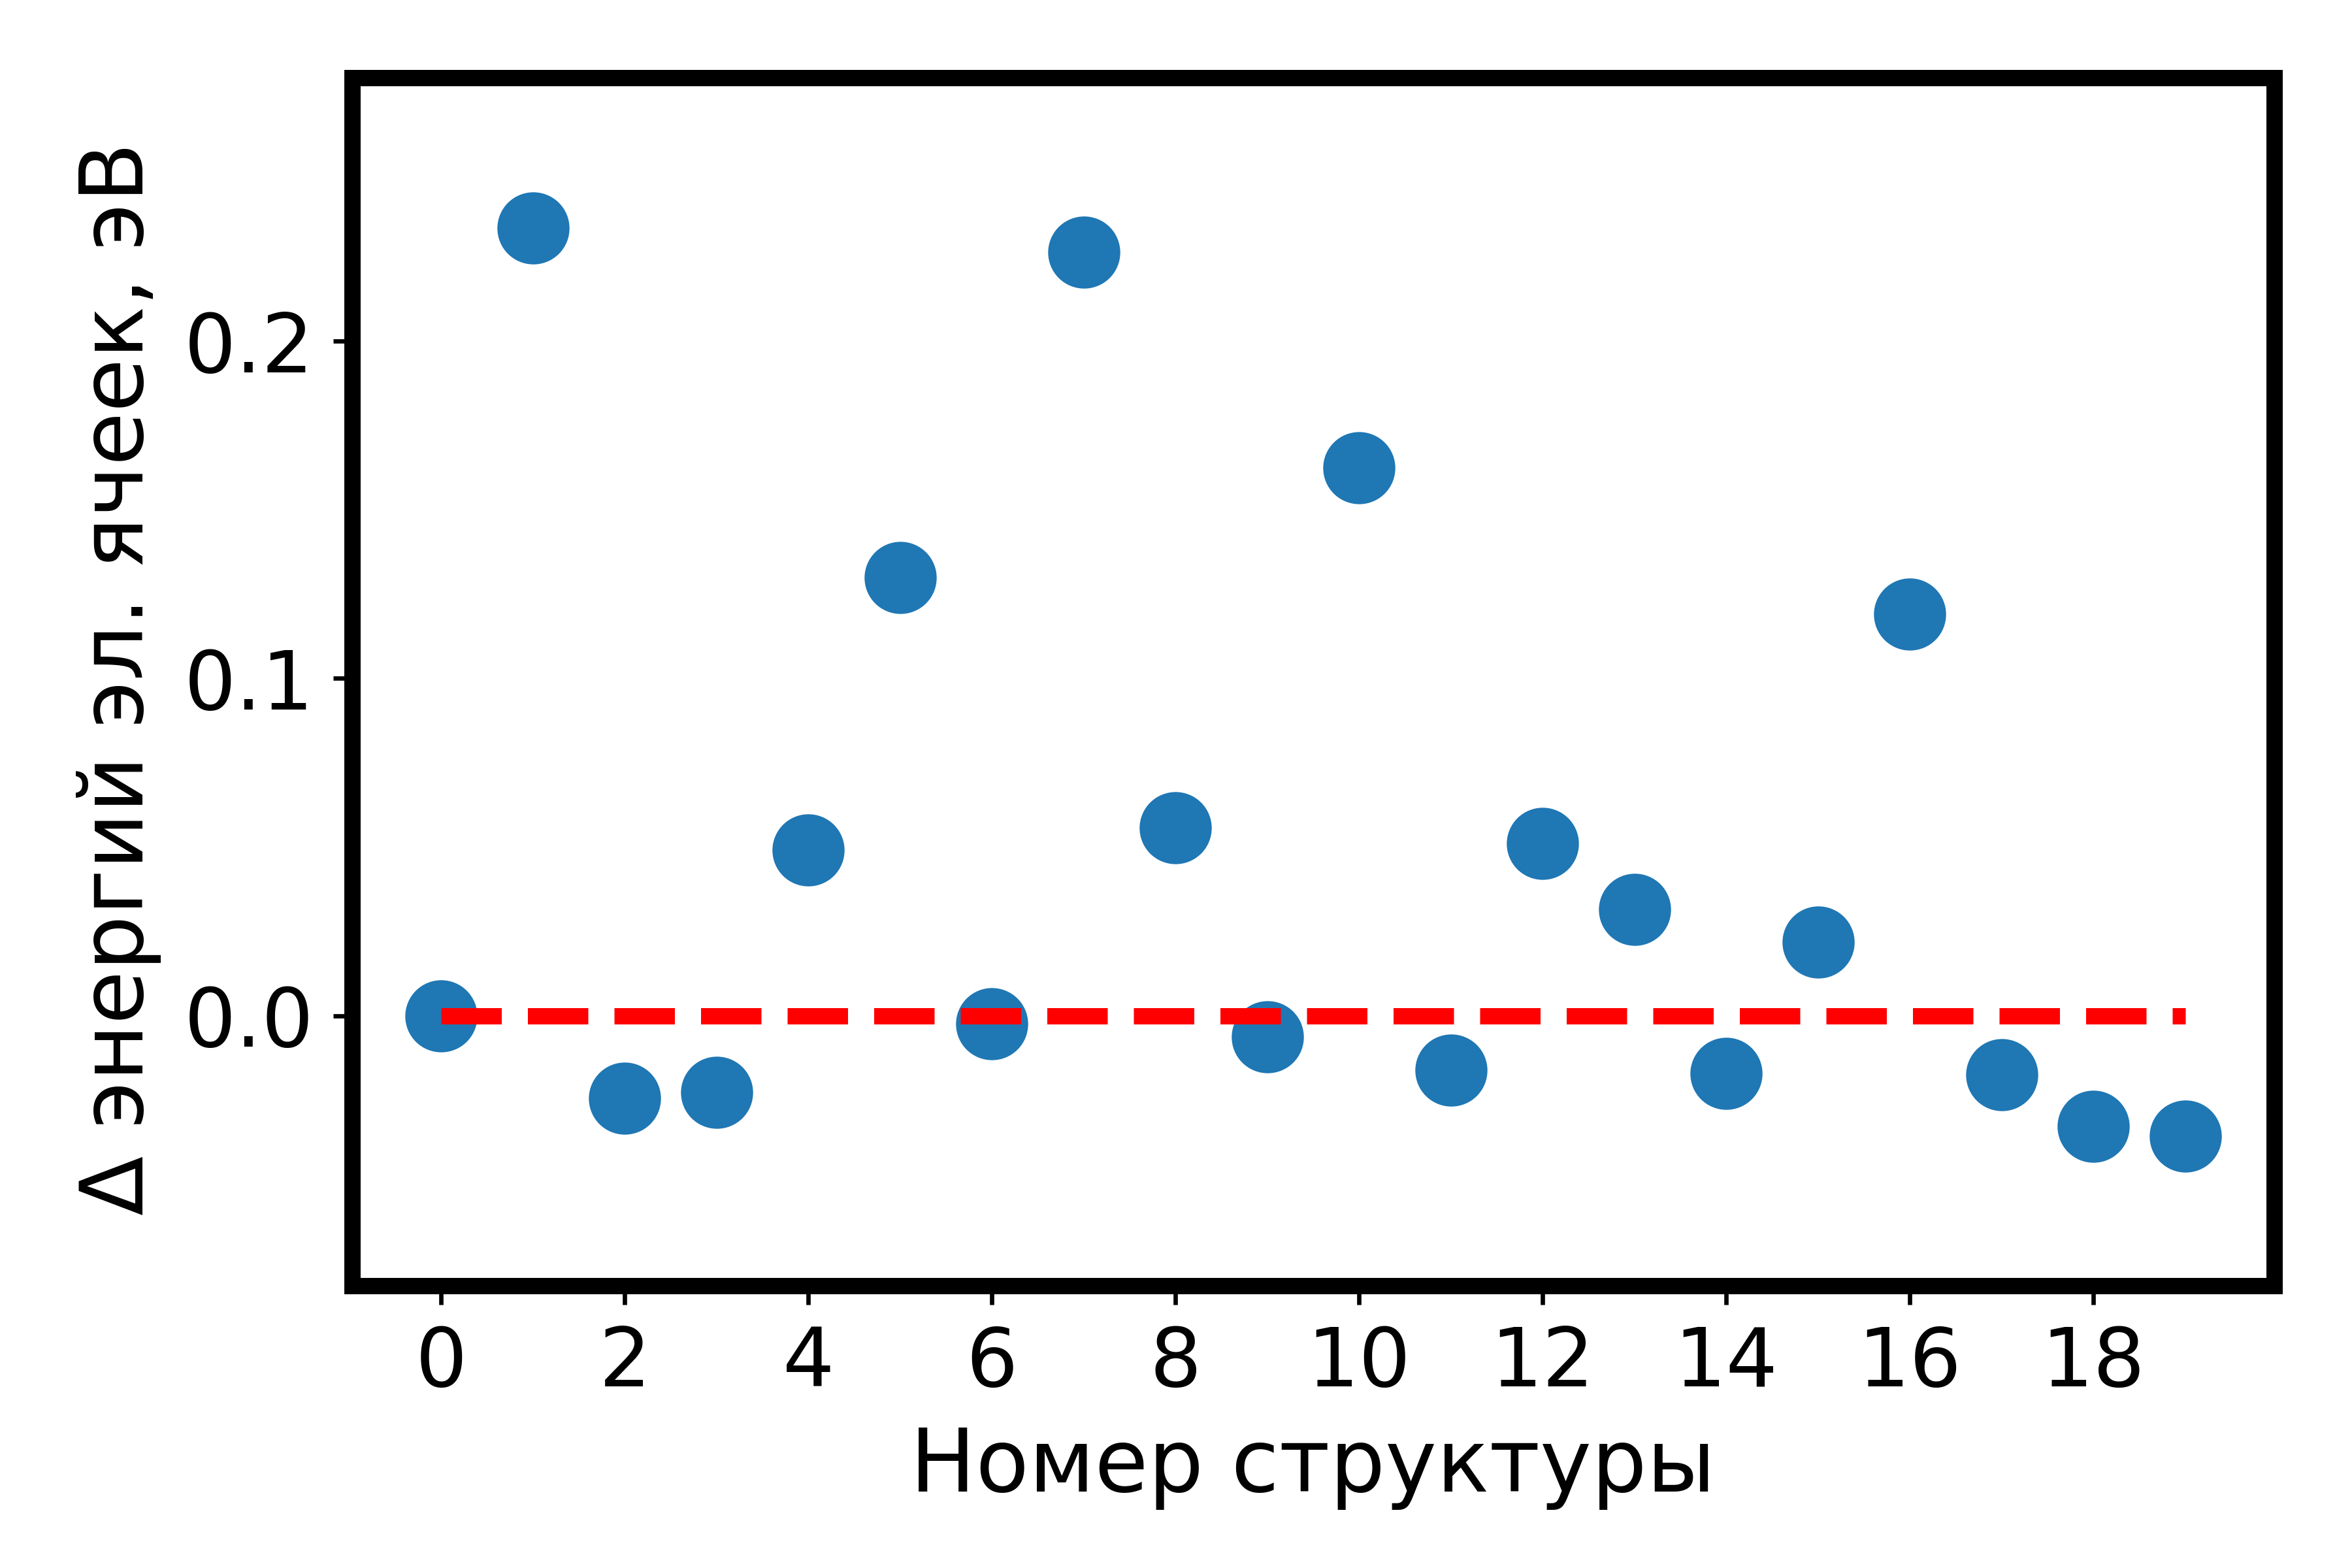
\includegraphics[width=0.7\linewidth]{energy_structure}
  \end{minipage}

      \caption[Сводный график энергий рассчитанных структур относительно энергии исходной структуры с разным расположением атомов в лавесовском полиэдре]{Сводный график энергий рассчитанных структур относительно энергии исходной структуры с разным расположением атомов в лавесовском полиэдре}
    \label{img:th}
\end{figure}

По результатам рентгеноструктурного анализа монокристаллического образца синтетического теннантита Cu\textsubscript{12}As\textsubscript{4}S\textsubscript{13} при комнатной температуре обнаружено, что значение суммы заселенностей позиций атомов Cu2 и Cu21 составляет 1, а не 1.04 как опубликовано ранее\cite{Makovicky_2006}.
Полученные результаты показывают, что на структурную формулу синтетического теннантита приходится 12 атомов меди, а не 12.5.
Таким образом, лавесовский полиэдр состоит из 6 атомов меди.
Наличие рядов меди с электронной плотностью в форме эллипса, определенное после анализа плоскости (011) атомарного изображения монокристаллического образца синтетического теннантита Cu\textsubscript{12}As\textsubscript{4}S\textsubscript{13} (Рис.~\ref{img:figure5}), показывает существование позиции атома меди Cu21 и согласуется с результатами рентгеноструктурного анализа, описанного выше.

По данным первопринципных расчётов энергий элементарных ячеек для синтетического теннантита Cu\textsubscript{12}As\textsubscript{4}S\textsubscript{13} следует,  что смещение атома меди в лавесовском полиэдре может приводить как к увеличению энергии ячейки, так и к уменьшению.
Результаты показывают, что существующее неэквивалентное  окружение атомов меди в позициях Cu21 и Cu2 ведет к отличию химического потенциала для структур с разным расположением атомов меди (анализировались позиции Cu21 и Cu2) и, вероятно, является движущей силой для возникновения позиции Cu21. Расстояние между сдвинутым атомом и его идеальным положением в лавесовском полиэдре составляет для наиболее энергетически выгодной элементарной ячейки 0.6~$\angstrom$, по экспериментальным данным --- 1.027(6)~$\angstrom$.
Анализ распределения электрических зарядов показывает, что для более выгодных с энергетической точки зрения структур не возникает разной валентности на атомах меди Cu1,
но появляется разность зарядов для позиций атомов Cu2 (Cu21) (варианты структур с 11 по 15). Также следует отметить, что структуры, где сдвинуты все 6 атомов меди, обладают большей энергией элементарной ячейки в сравнении с энергией идеального полиэдра и имеют не самые энергетически выгодные конфигурации  (варианты 5--10).

На рисунке \ref{img:xray2} показаны изображения распределений электронной плотности синтетического теннантита Cu\textsubscript{12}As\textsubscript{4}S\textsubscript{13} при температуре 293~(а) и 85~(б)~К в плоскости (011).
По форме сечений линий электронной плотности видно, что происходит полное разделение позиций Cu2 и Cu21.
При комнатной температуре расстояние между Cu2 и Cu21 составляет 1.027(6)~$\angstrom$, при 85~К --- 1.108(5)~$\angstrom$.
Расчёт энергий ФМ, АФМ, ПМ и диамагнитного состояний для экспериментально полученных структур показывает, что АФМ упорядочение в экспериментальной структуре при 85~К энергетически более выгодно, чем ферро-, пара- или диамагнитное состояния при этой же температуре.
Для экспериментальной структуры при 293~К ФМ, АФМ, ПМ конфигурации имеют одинаковую до (4 знака) энергию, что указывает на их одинаковую вероятность.

\begin{figure}[hb]
  \begin{minipage}[ht]{0.5\linewidth}\centering
    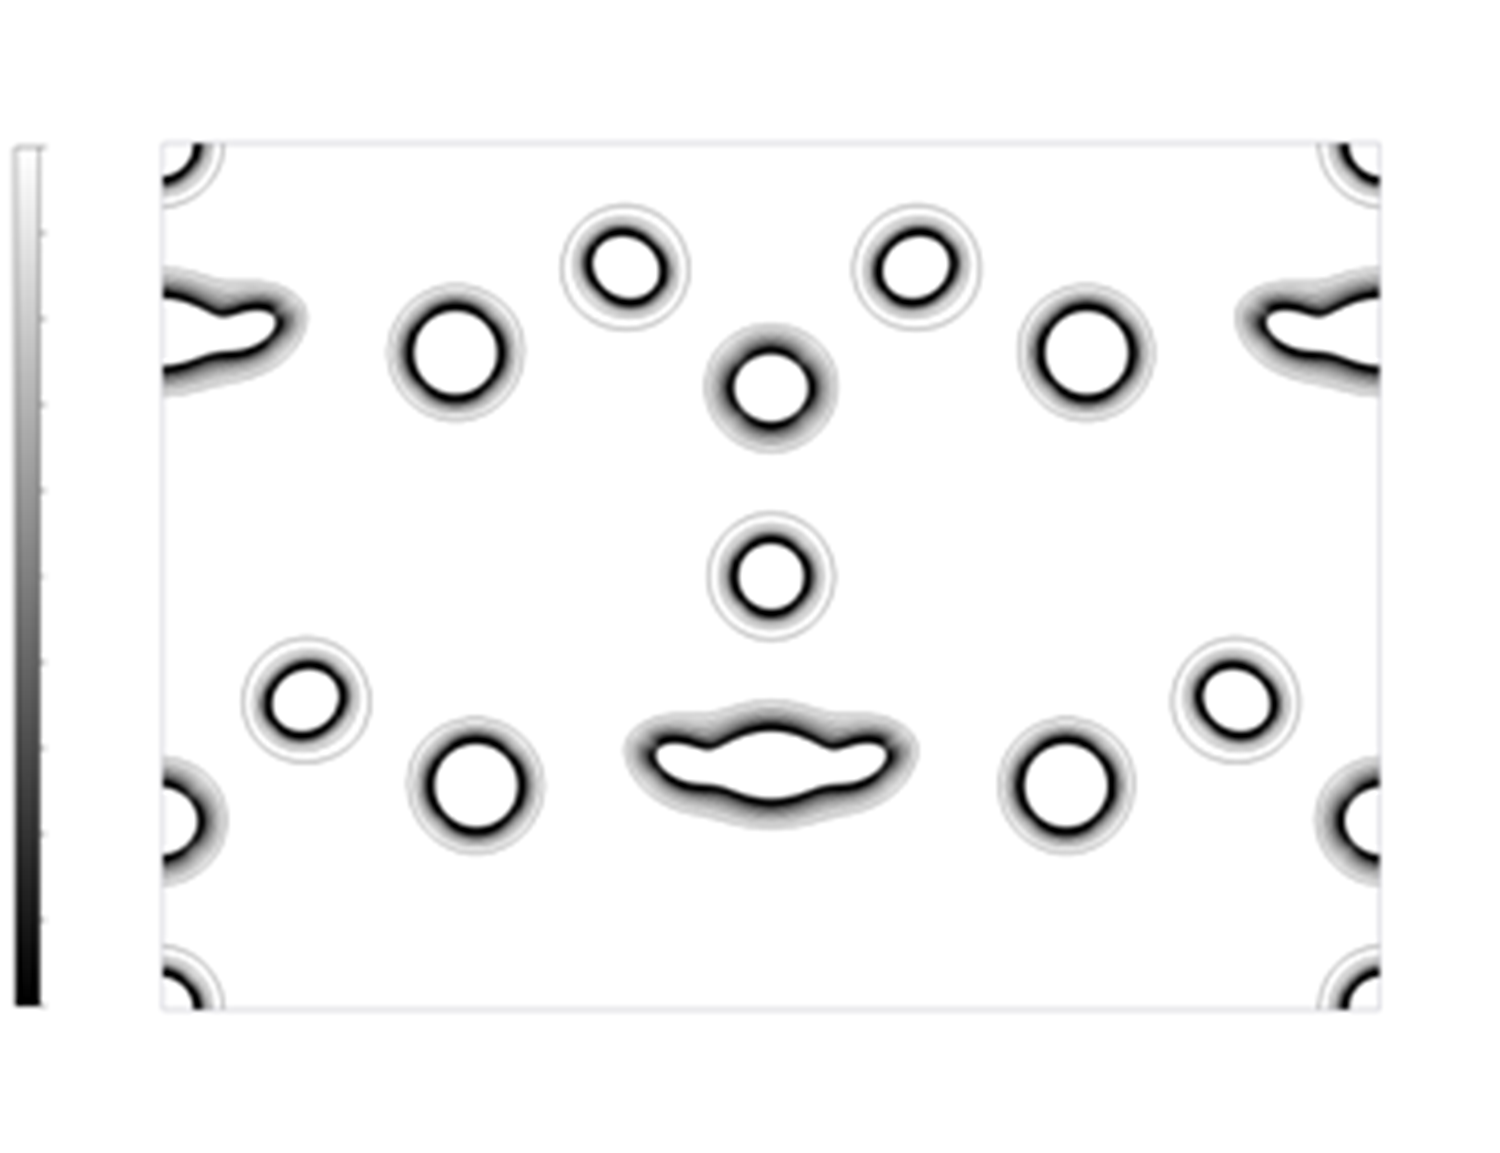
\includegraphics[width=0.9\linewidth]{Electron_density_293.png} \\ а)
  \end{minipage}
  \hfill
  \begin{minipage}[ht]{0.5\linewidth}\centering
    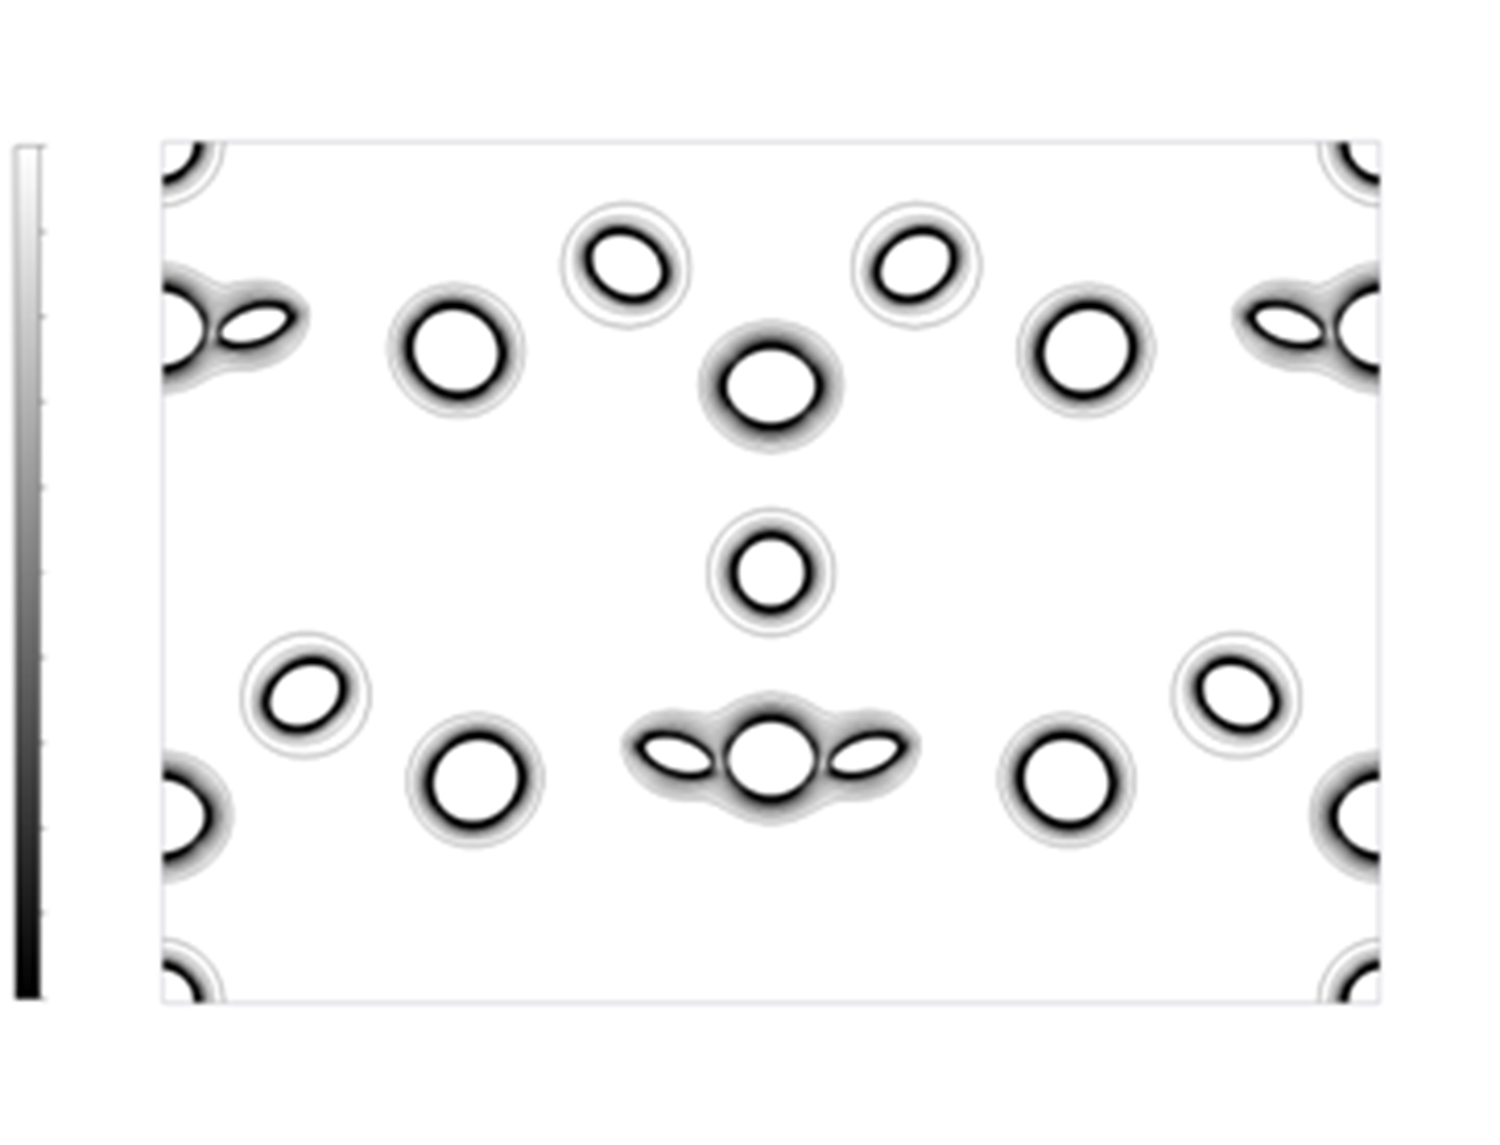
\includegraphics[width=0.9\linewidth]{Electron_density_85.png} \\ б)
  \end{minipage}

      \caption[Распределение электронной плотности при температуре 293~(а) и 85~(б)~К в плоскости (011) синтетического теннантита Cu\textsubscript{12}As\textsubscript{4}S\textsubscript{13}]{Распределение электронной плотности при температуре 293~(а) и 85~(б)~К в плоскости (011) синтетического теннантита Cu\textsubscript{12}As\textsubscript{4}S\textsubscript{13}}
    \label{img:xray2}
\end{figure}

В \underline{\textbf{четвёртой главе}} представлены результаты экспериментальных исследований зависимостей намагниченности в диапазоне температур от 2 до 350~К и спектров комбинационного рассеяния света для соединений Cu\textsubscript{12}As\textsubscript{4}S\textsubscript{13}, Cu\textsubscript{12}Sb\textsubscript{4}S\textsubscript{13}, Cu\textsubscript{3}AsSe\textsubscript{3} и Cu\textsubscript{3}SbSe\textsubscript{3} при комнатной температуре. А также измерения теплоёмкости в диапазоне температур от 4 до 350~К и результаты моделирования теплоёмкости для Cu\textsubscript{12}As\textsubscript{4}S\textsubscript{13} и Cu\textsubscript{3}AsSe\textsubscript{3}.

На рисунке \ref{img:figure4} представлены результаты расчётной и экспериментальной температурных зависимостей для синтетических теннантита Cu\textsubscript{12}As\textsubscript{4}S\textsubscript{13} и мгриита Cu\textsubscript{3}AsSe\textsubscript{3}.

 Температура Дебая при вычислении теплоёмкости для синтетического теннантита Cu\textsubscript{12}As\textsubscript{4}S\textsubscript{13} принята $\theta$\textsubscript{д}~=~623~К на основе лучшего соответствия расчетной  и экспериментальной  теплоёмкостей. Значения характеристических температур для осцилляторов Эйнштейна составляют $\theta$\textsubscript{э1}~=~220~К, $\theta$\textsubscript{э2}~=~124~К и $\theta$\textsubscript{э3}~=~41~К.
Температура Дебая при вычислении теплоёмкости для синтетического мгриита принята Cu\textsubscript{3}AsSe\textsubscript{3} $\theta$\textsubscript{д}~=~500~К  на основе лучшего соответствия расчетной  и экспериментальной  теплоёмкостей. Значения для осцилляторов Эйнштейна составляют $\theta$\textsubscript{э1}~=~290~К, $\theta$\textsubscript{э2}~=~185~К и $\theta$\textsubscript{э3}~=~44 К, которые определены из температурных зависимостей удельной намагниченности и литературных данных.

\begin{figure}[ht]
  \begin{minipage}[ht]{0.5\linewidth}\centering
    \includegraphics[width=0.9\linewidth]{Heat_capacity_Cu12As4S13} \\ а)
  \end{minipage}
  \hfill
  \begin{minipage}[ht]{0.5\linewidth}\centering
    \includegraphics[width=0.9\linewidth]{Heat_capacity_Cu3AsSe3} \\ б)
  \end{minipage}

      \caption[Зависимость теплоёмкости образцов Cu\textsubscript{12}As\textsubscript{4}S\textsubscript{13}(а) и Cu\textsubscript{3}AsS\textsubscript{3}(б) от температуры. Точки~"---экспериментальные данные, сплошная линия~"---модельные значения теплоёмкости, пунктиром отмечен уровень доверия 95\% ]{Зависимость теплоёмкости образцов Cu\textsubscript{12}As\textsubscript{4}S\textsubscript{13}(а) и Cu\textsubscript{3}AsS\textsubscript{3}(б) от температуры. Точки~"---экспериментальные данные, сплошная линия~"---модельные значения теплоёмкости, пунктиром отмечен уровень доверия 95\%}
    \label{img:figure4}
\end{figure}

Спектры комбинационного рассеяния для исследованных соединений обладают низкоэнергетическими модами (Рис. \ref{img:figure_raman}).
В таблице \ref{tabl_raman} представлены определенные по экспериментальным спектрам положения пиков для исследуемых соединений и их полуширина.
Следует отметить, что энергия пиков для соединения Cu\textsubscript{12}Sb\textsubscript{4}S\textsubscript{13} составляет 8.5  и 12~мэВ, что наxодится в хорошем согласии с опубликованными теоретическими\cite{Lai_2015} и экспериментальными\cite{May2016}  данными.

Определение положения  и  полуширины пика проведены с помощью функции псевдо-Фойгта.
Модель аппроксимации  основана на функциях псевдо-Фойгта для каждого пика и полиномной функции для фона.

\begin{table} [t!]%
    \centering
	\caption{Положение пиков на спектрах комбинационного рассеяния и их полуширина для сложных соединений халькогенидов меди}%
	\label{tabl_raman}% label всегда желательно идти после caption
    \renewcommand{\arraystretch}{1.5}
	\begin{tabular}{@{}@{\extracolsep{20pt}}lllll@{}}
        \toprule     %%% верхняя линейка
    	 & \multicolumn{3}{c}{положение пика и  полуширина, см\textsuperscript{-1}}& \\
        \midrule
    Cu\textsubscript{12}As\textsubscript{4}S\textsubscript{13} & 67 (14)	 &122 (24) 											& & 	\\ \hline
   Cu\textsubscript{3}AsSe\textsubscript{3}&  155 (7)				& 200 (37)						&254 (6) 	&  \\ \hline
    	 Cu\textsubscript{12}Sb\textsubscript{4}S\textsubscript{13} 	& 69 (20)	& 97 (11) 	& 		& 	\\ \hline
    	 Cu\textsubscript{3}SbSe\textsubscript{3}	 	& 110 (14)				& 148 (11) 	& 205 (25)		& \\ \hline
        \bottomrule
	\end{tabular}%
\end{table}



\begin{figure}[b!]
  \begin{minipage}[ht]{0.5\linewidth}\centering
    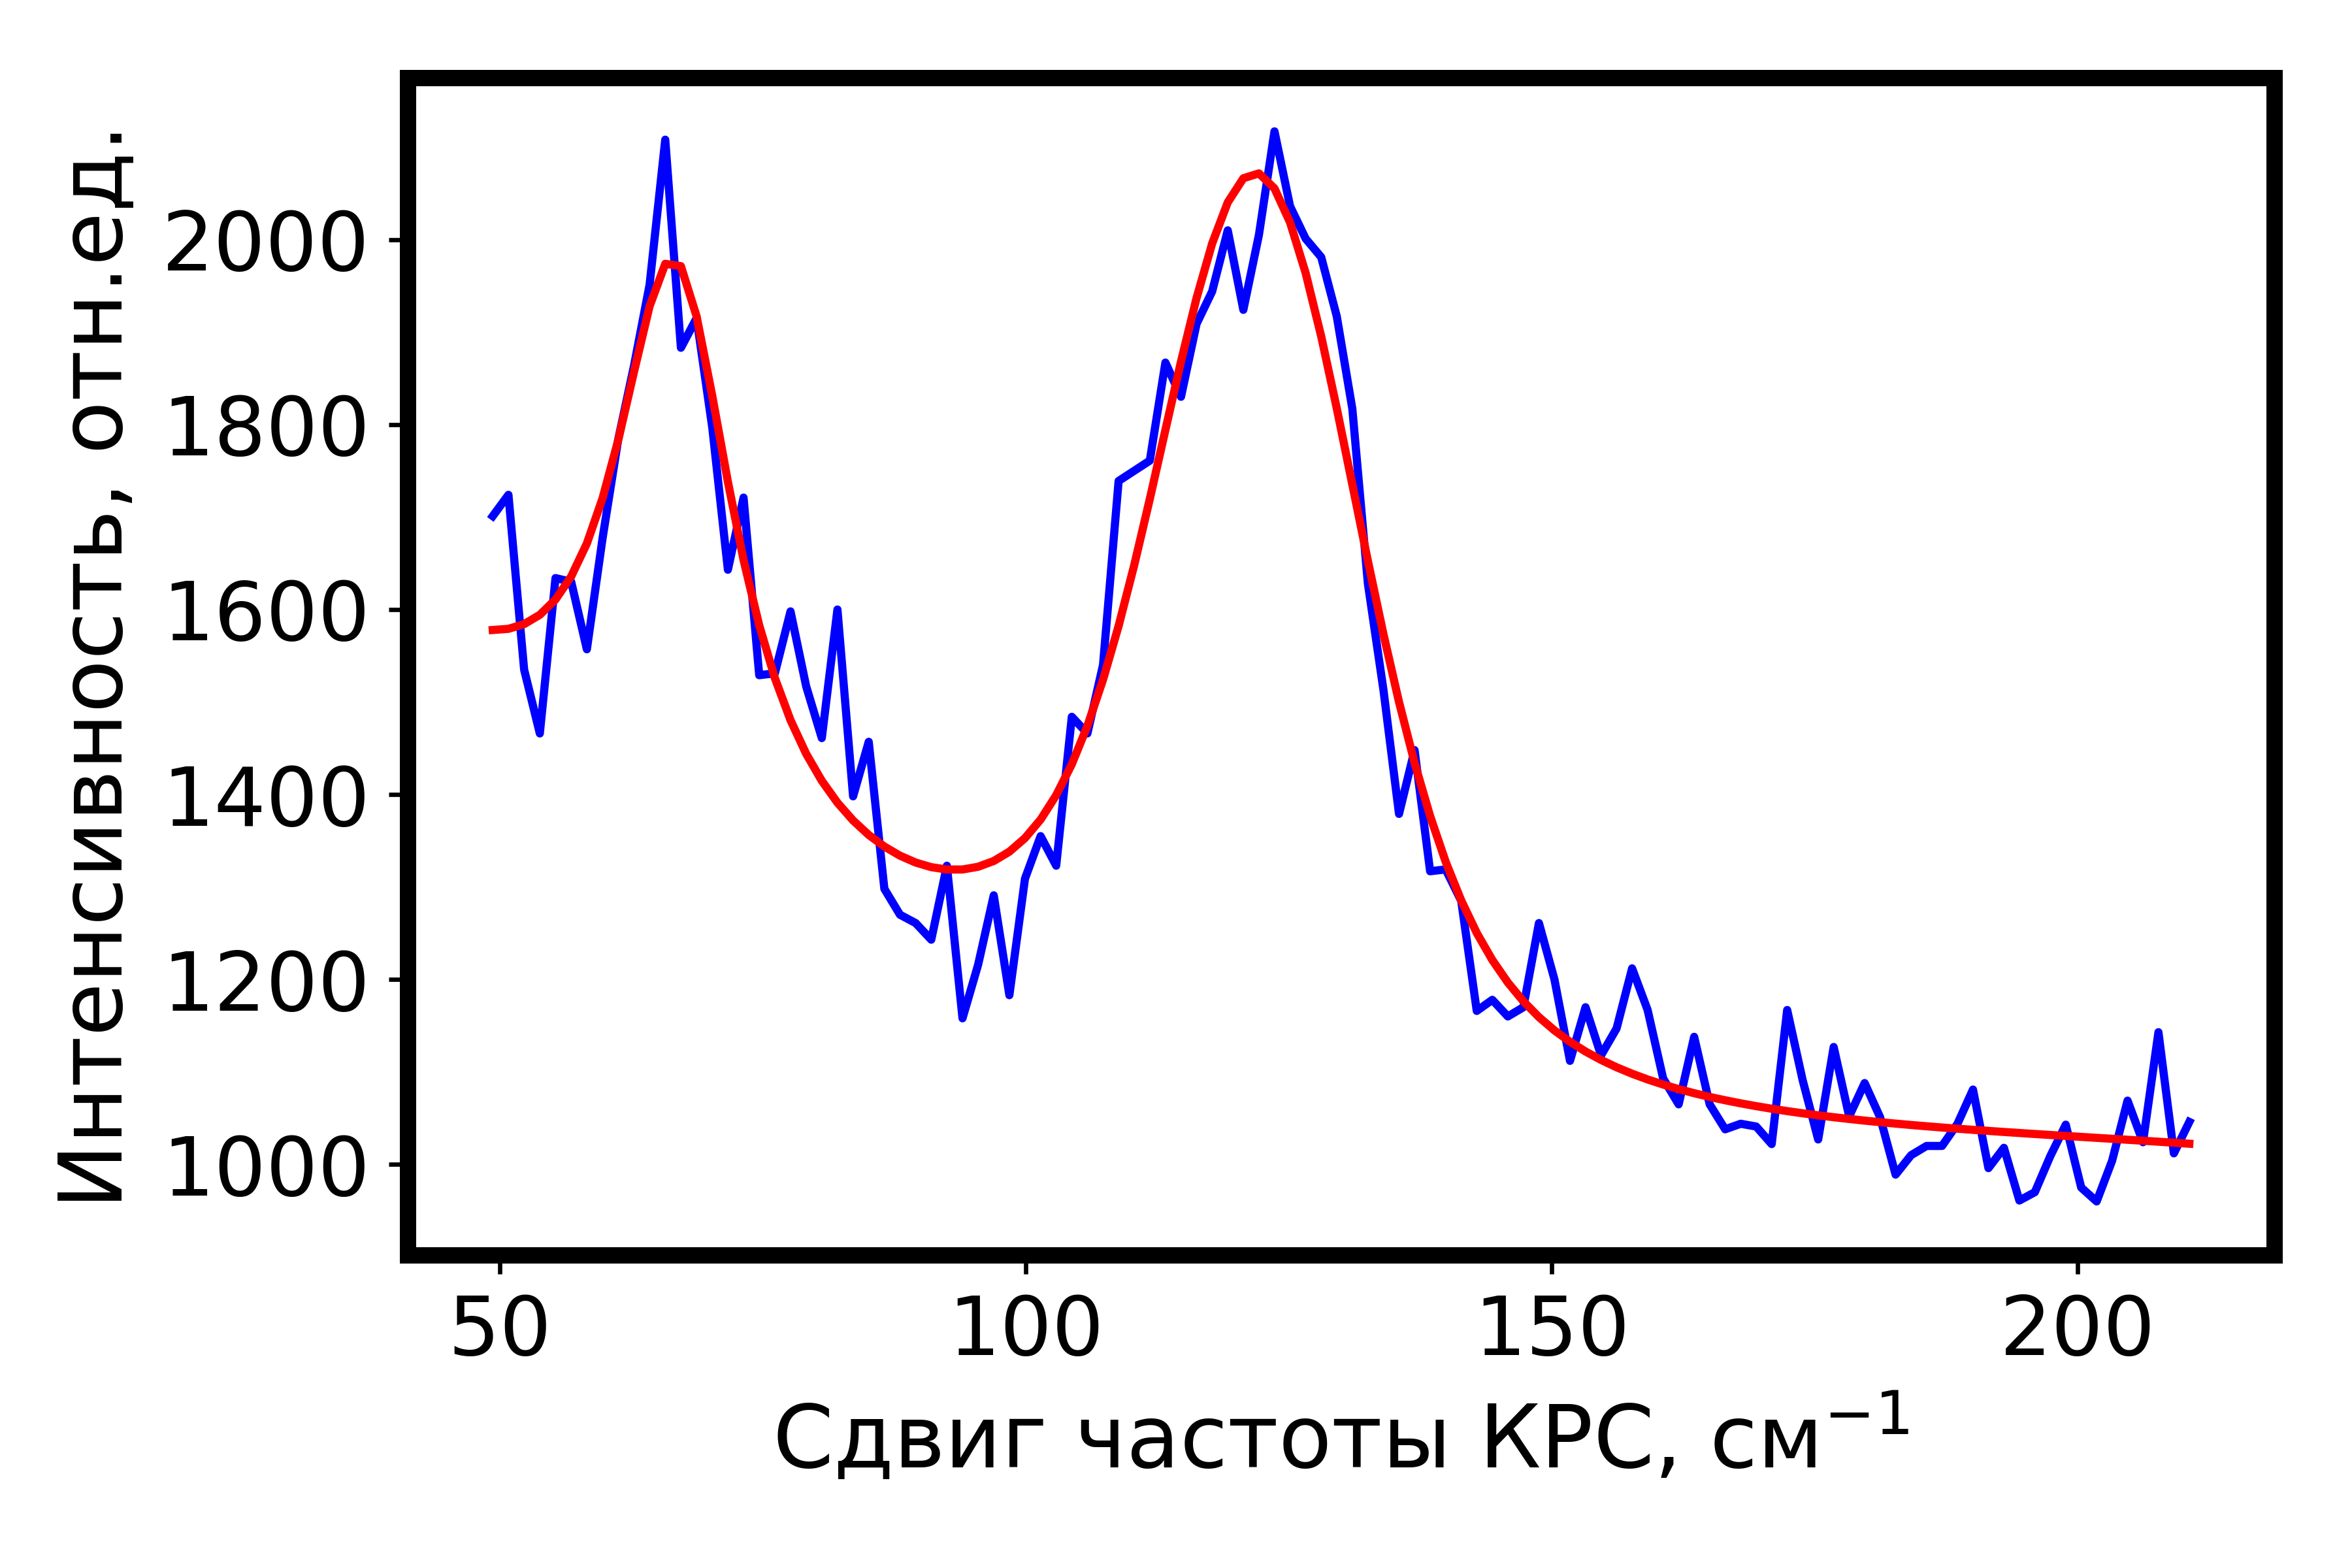
\includegraphics[width=0.9\linewidth]{raman_25_CuAsS3} \\ а)
  \end{minipage}
  \hfill
  \begin{minipage}[ht]{0.5\linewidth}\centering
    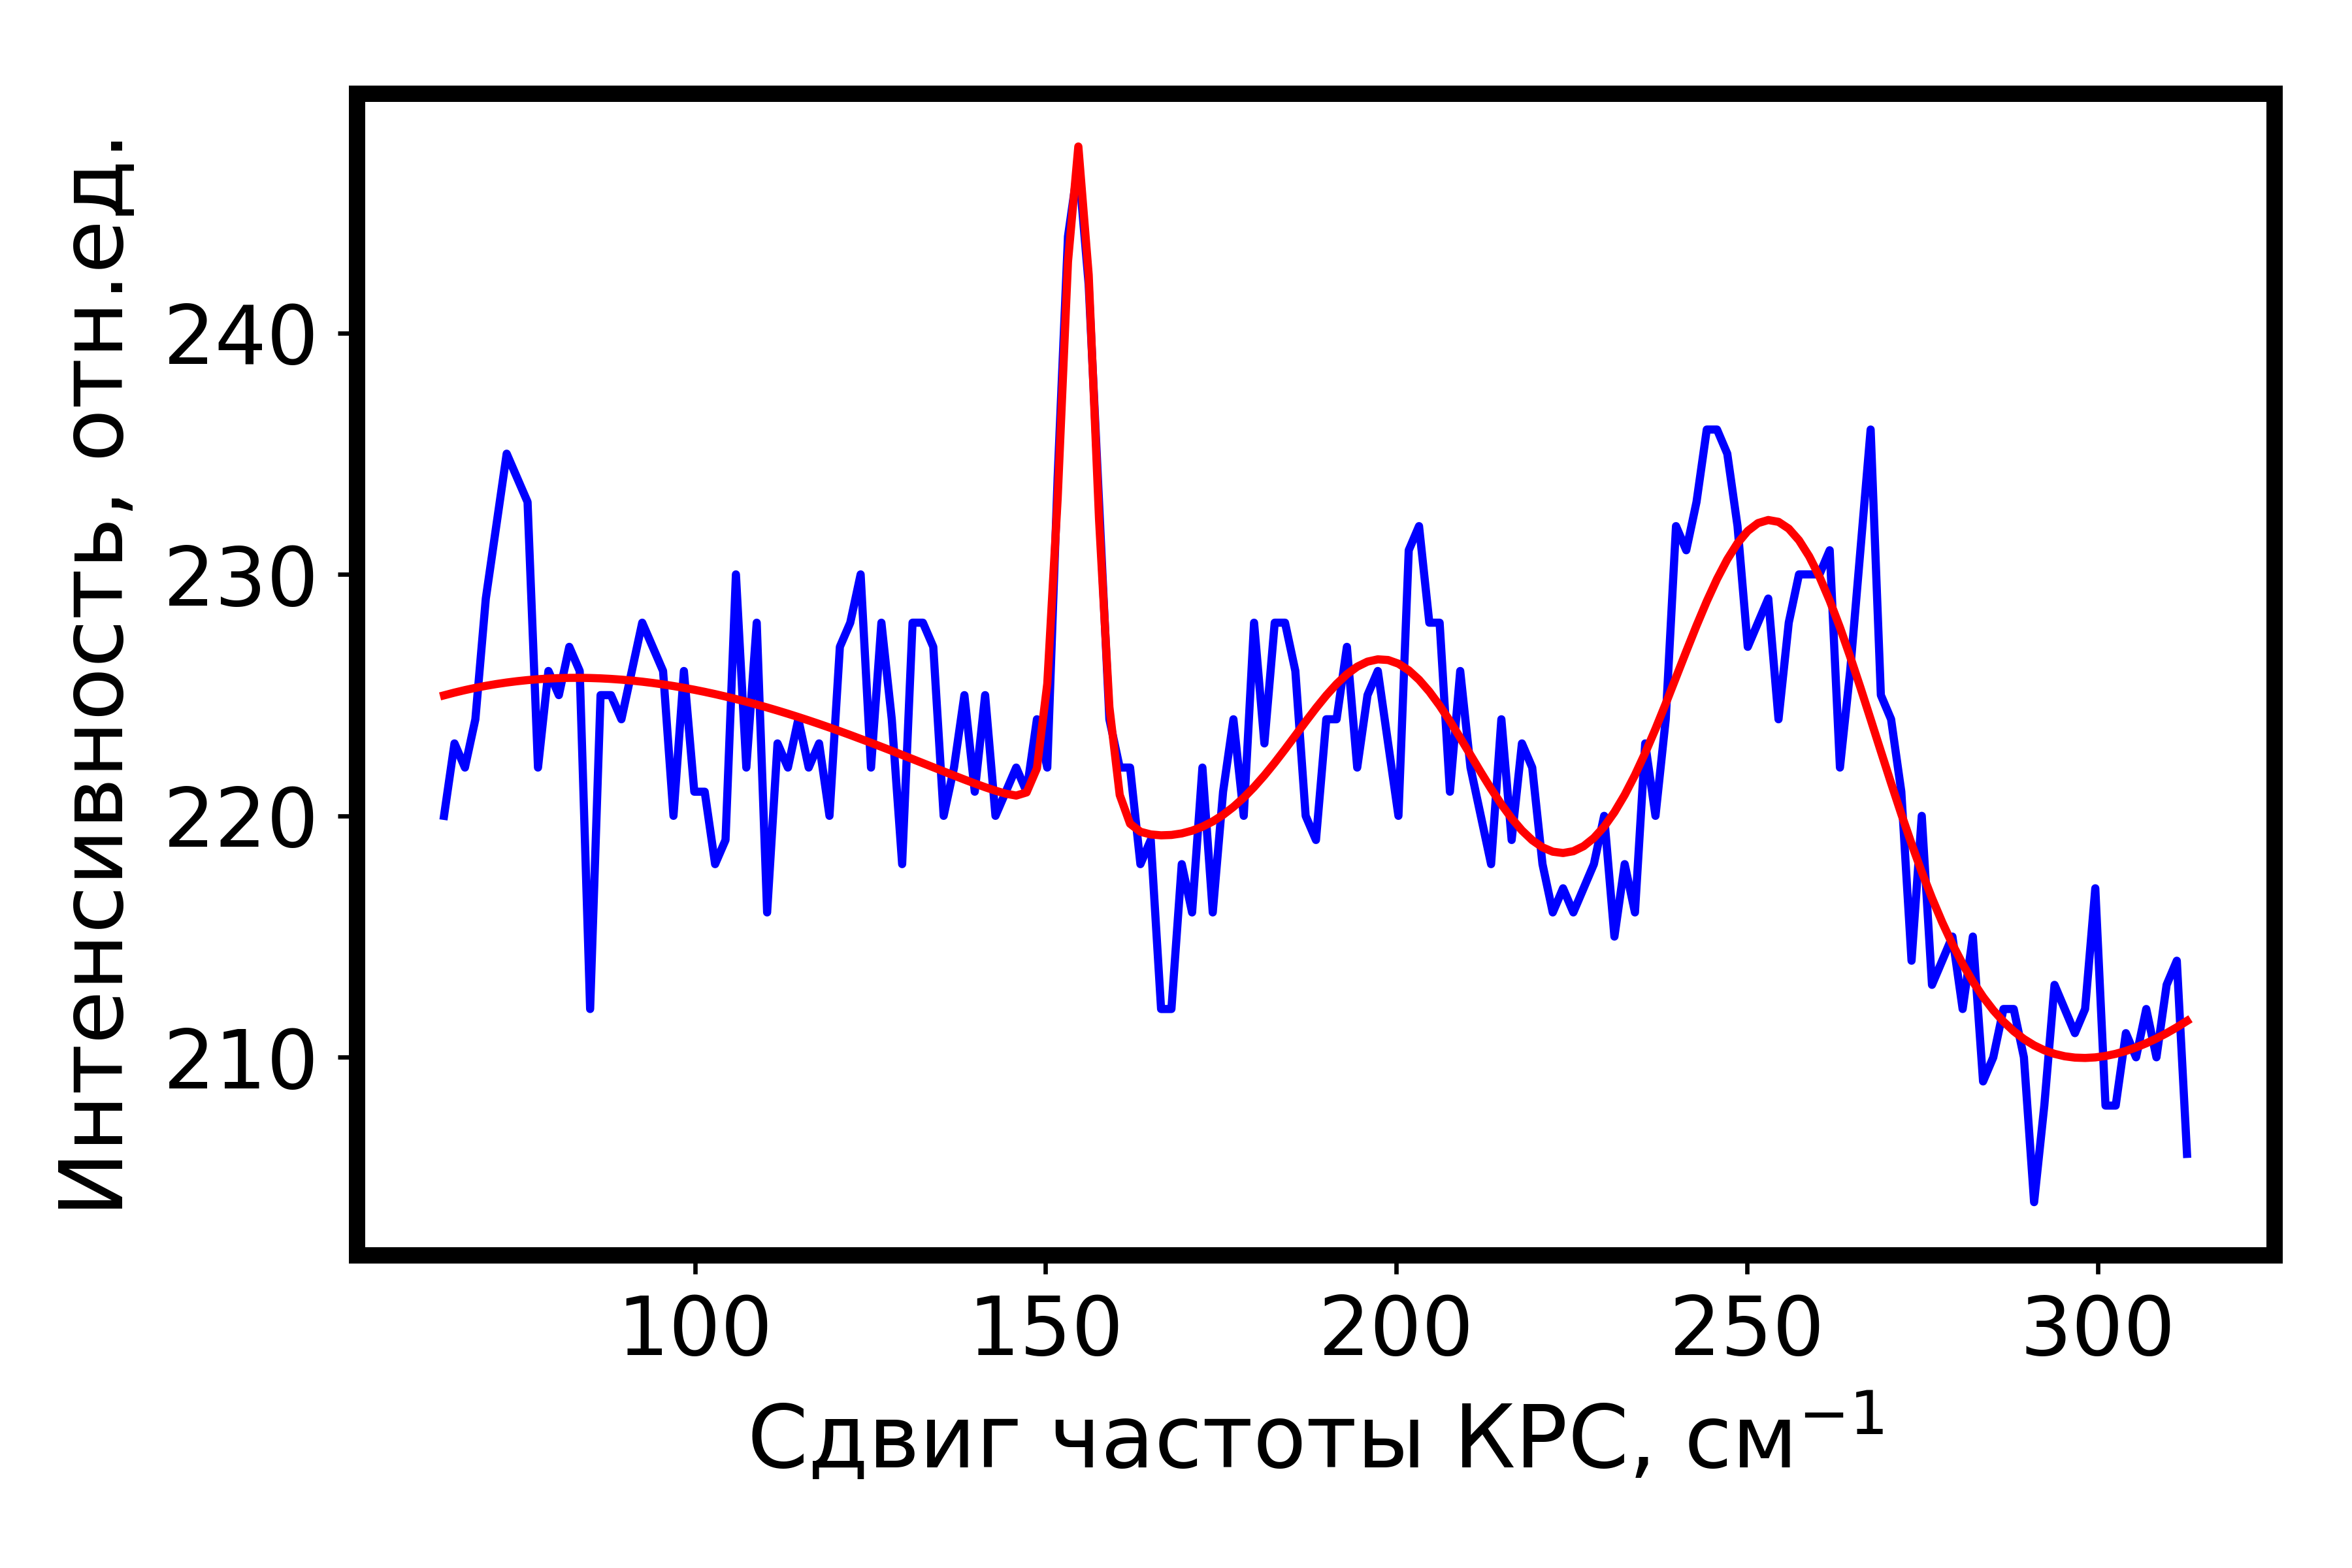
\includegraphics[width=0.9\linewidth]{raman_288_Cu3AsSe3} \\ б)
  \end{minipage}
\vfill
  \begin{minipage}[ht]{0.5\linewidth}\centering
    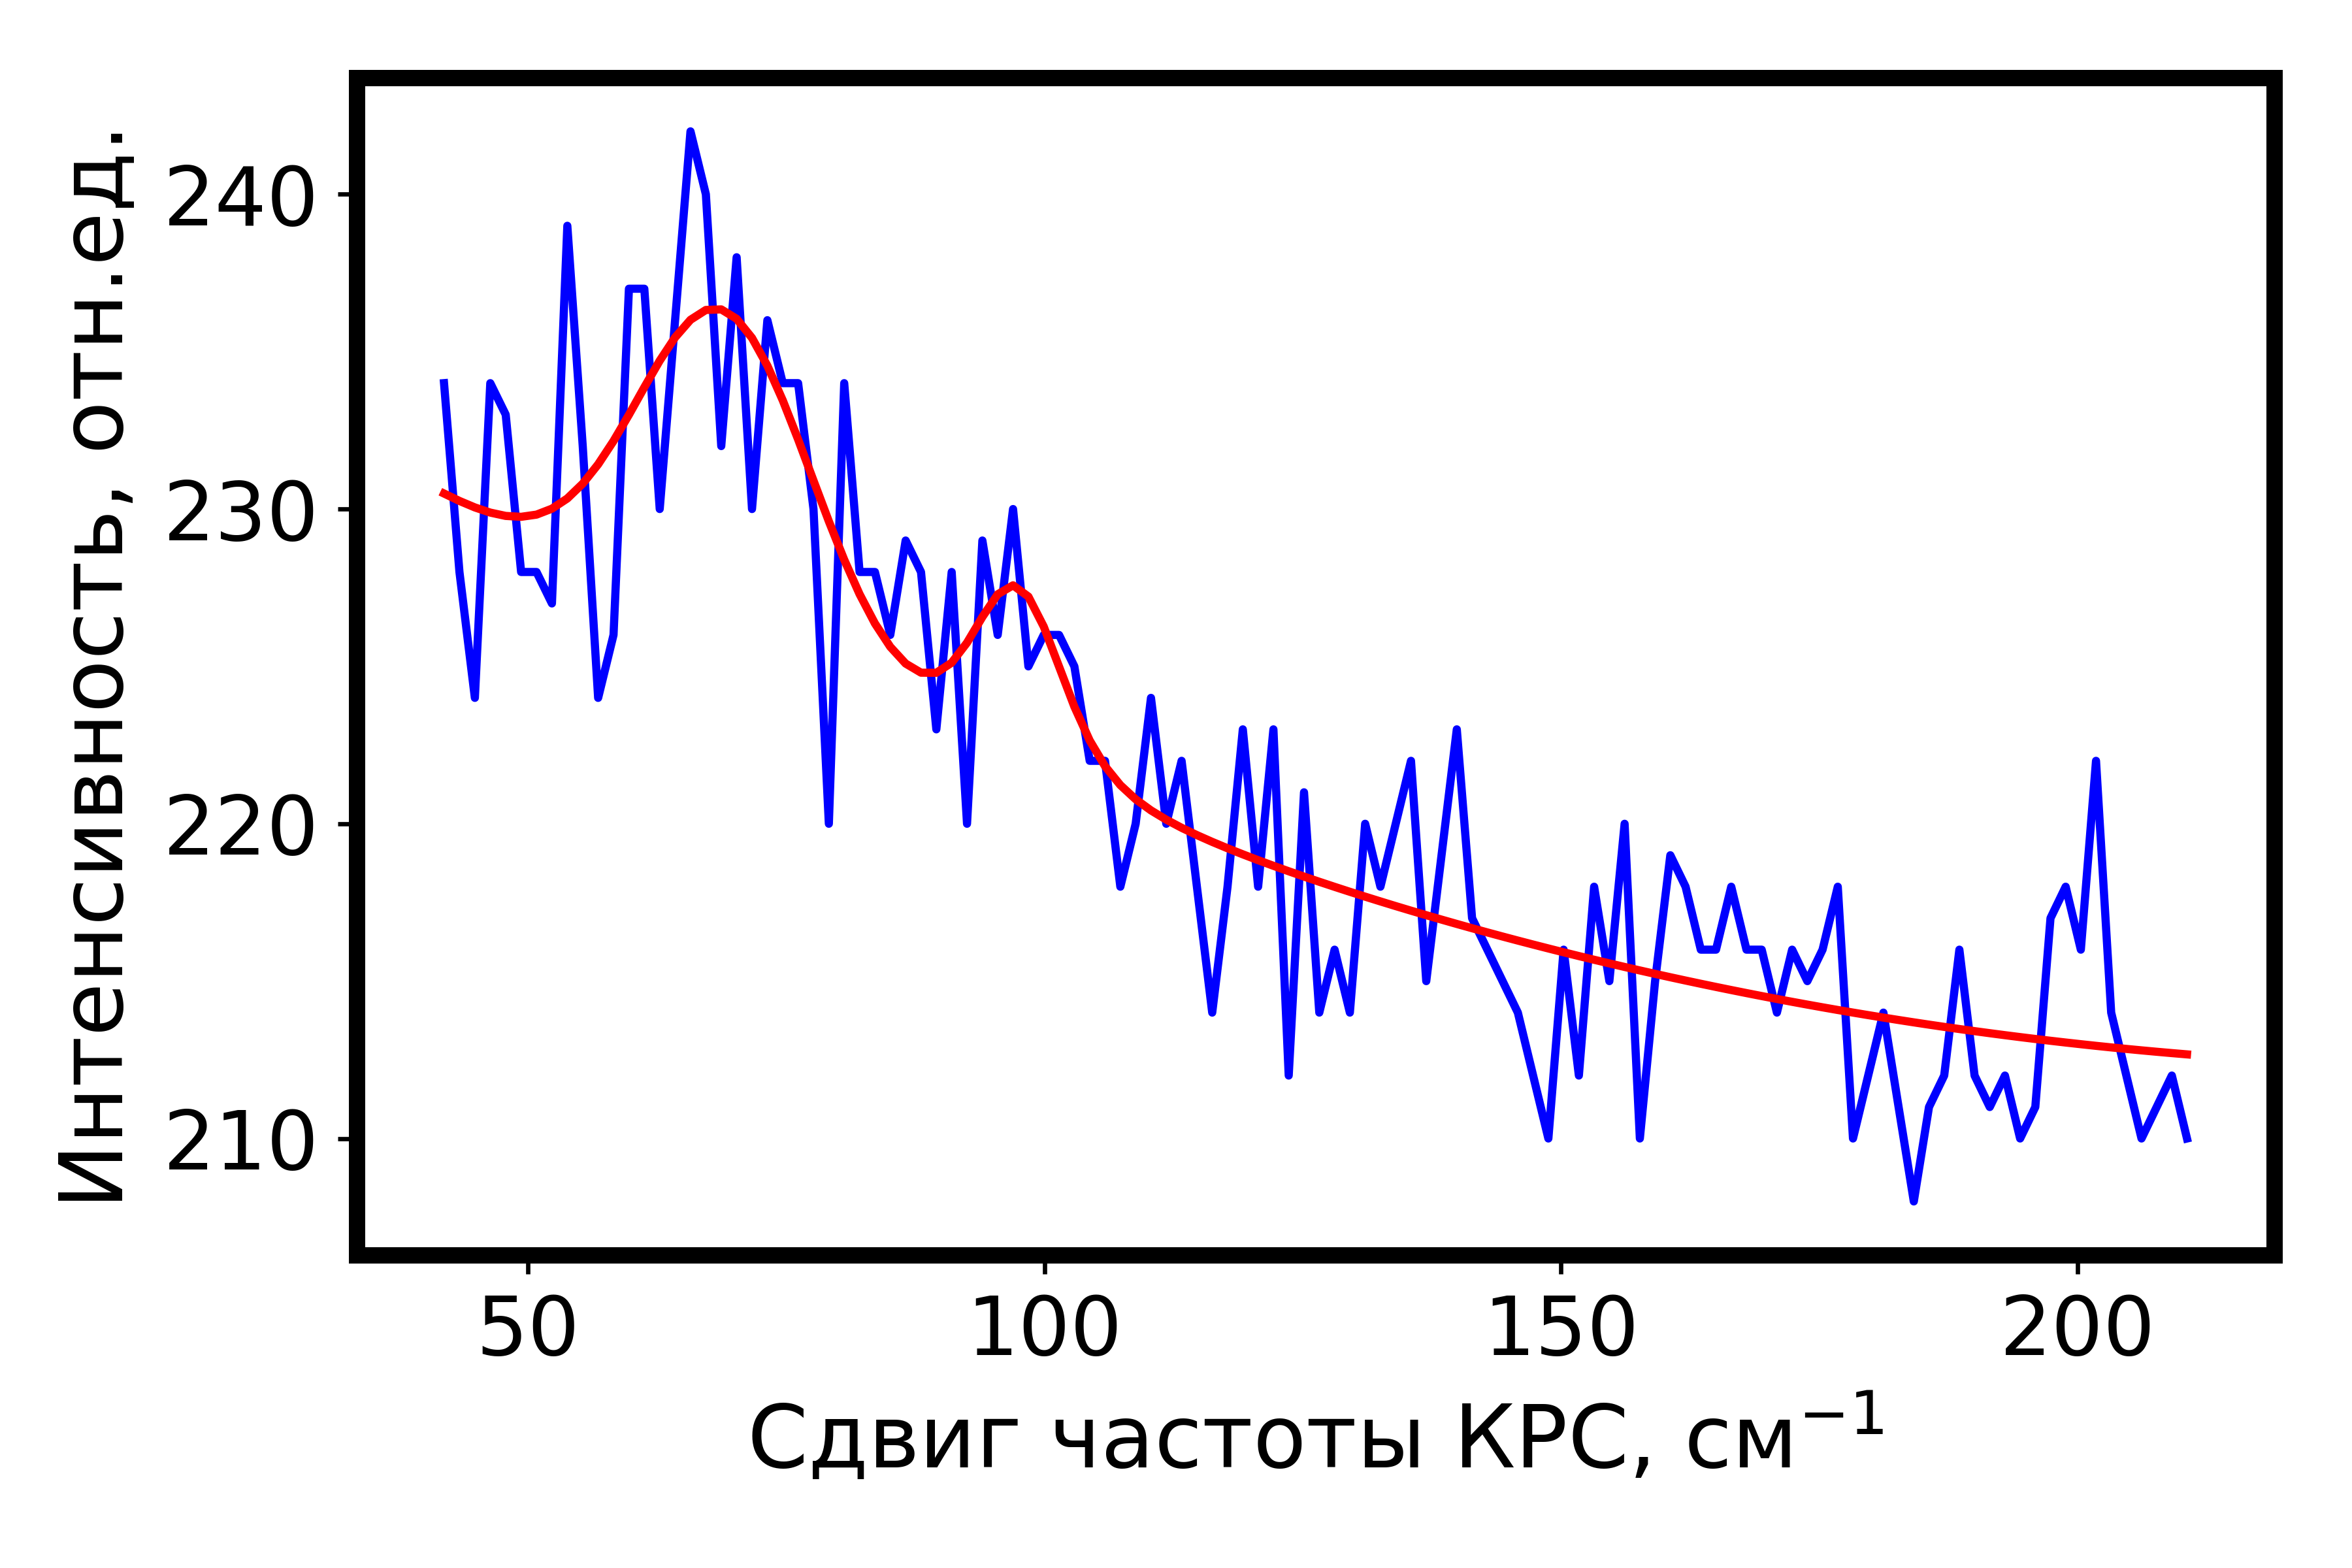
\includegraphics[width=0.9\linewidth]{raman_206_Cu3SbS3} \\ в)
  \end{minipage}
  \hfill
  \begin{minipage}[ht]{0.5\linewidth}\centering
    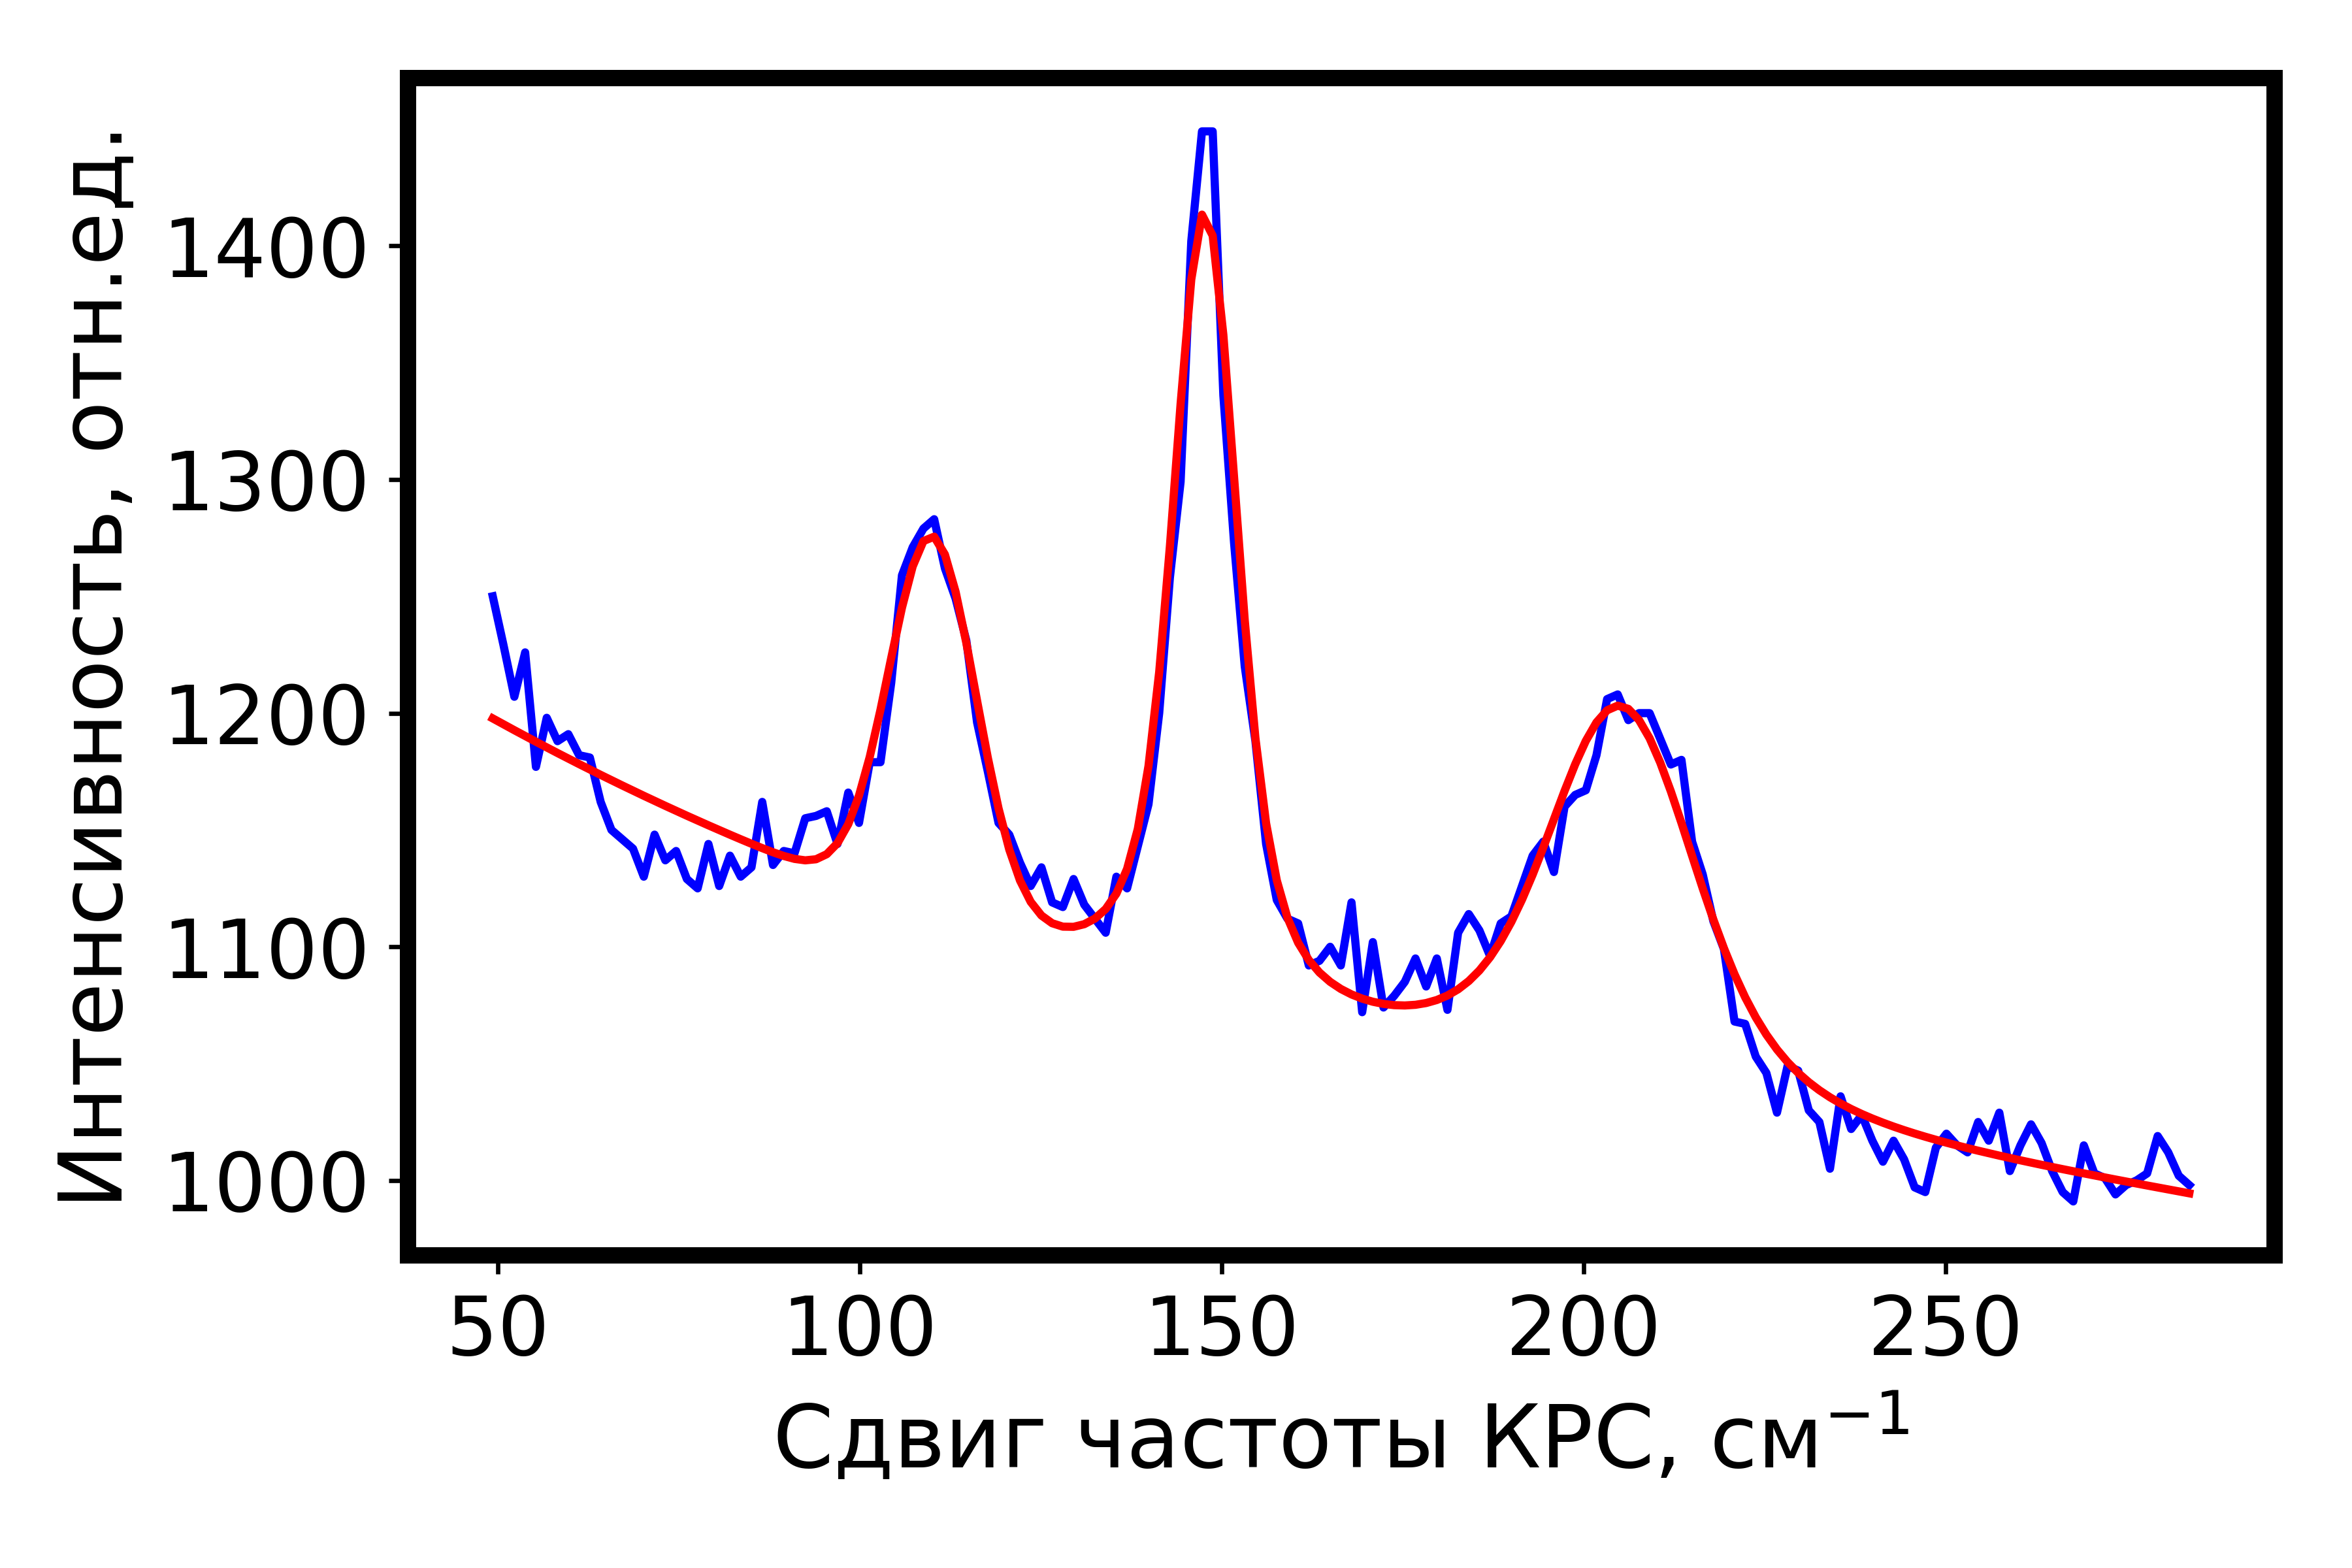
\includegraphics[width=0.9\linewidth]{raman_209_Cu3SbSe3} \\ г)
  \end{minipage}

      \caption[Графики спектров комбинационного рассеяния соединений Cu\textsubscript{12}As\textsubscript{4}S\textsubscript{13} (а), Cu\textsubscript{12}Sb\textsubscript{4}S\textsubscript{13} (б), Cu\textsubscript{3}AsSe\textsubscript{3} (в) и Cu\textsubscript{3}SbSe\textsubscript{3} (г)]{Графики спектров комбинационного рассеяния соединений Cu\textsubscript{12}As\textsubscript{4}S\textsubscript{13} (а), Cu\textsubscript{12}Sb\textsubscript{4}S\textsubscript{13} (б), Cu\textsubscript{3}AsSe\textsubscript{3} (в) и Cu\textsubscript{3}SbSe\textsubscript{3} (г)}
    \label{img:figure_raman}
\end{figure}


\begin{figure}[b!]
  \begin{minipage}[ht]{0.5\linewidth}\centering
    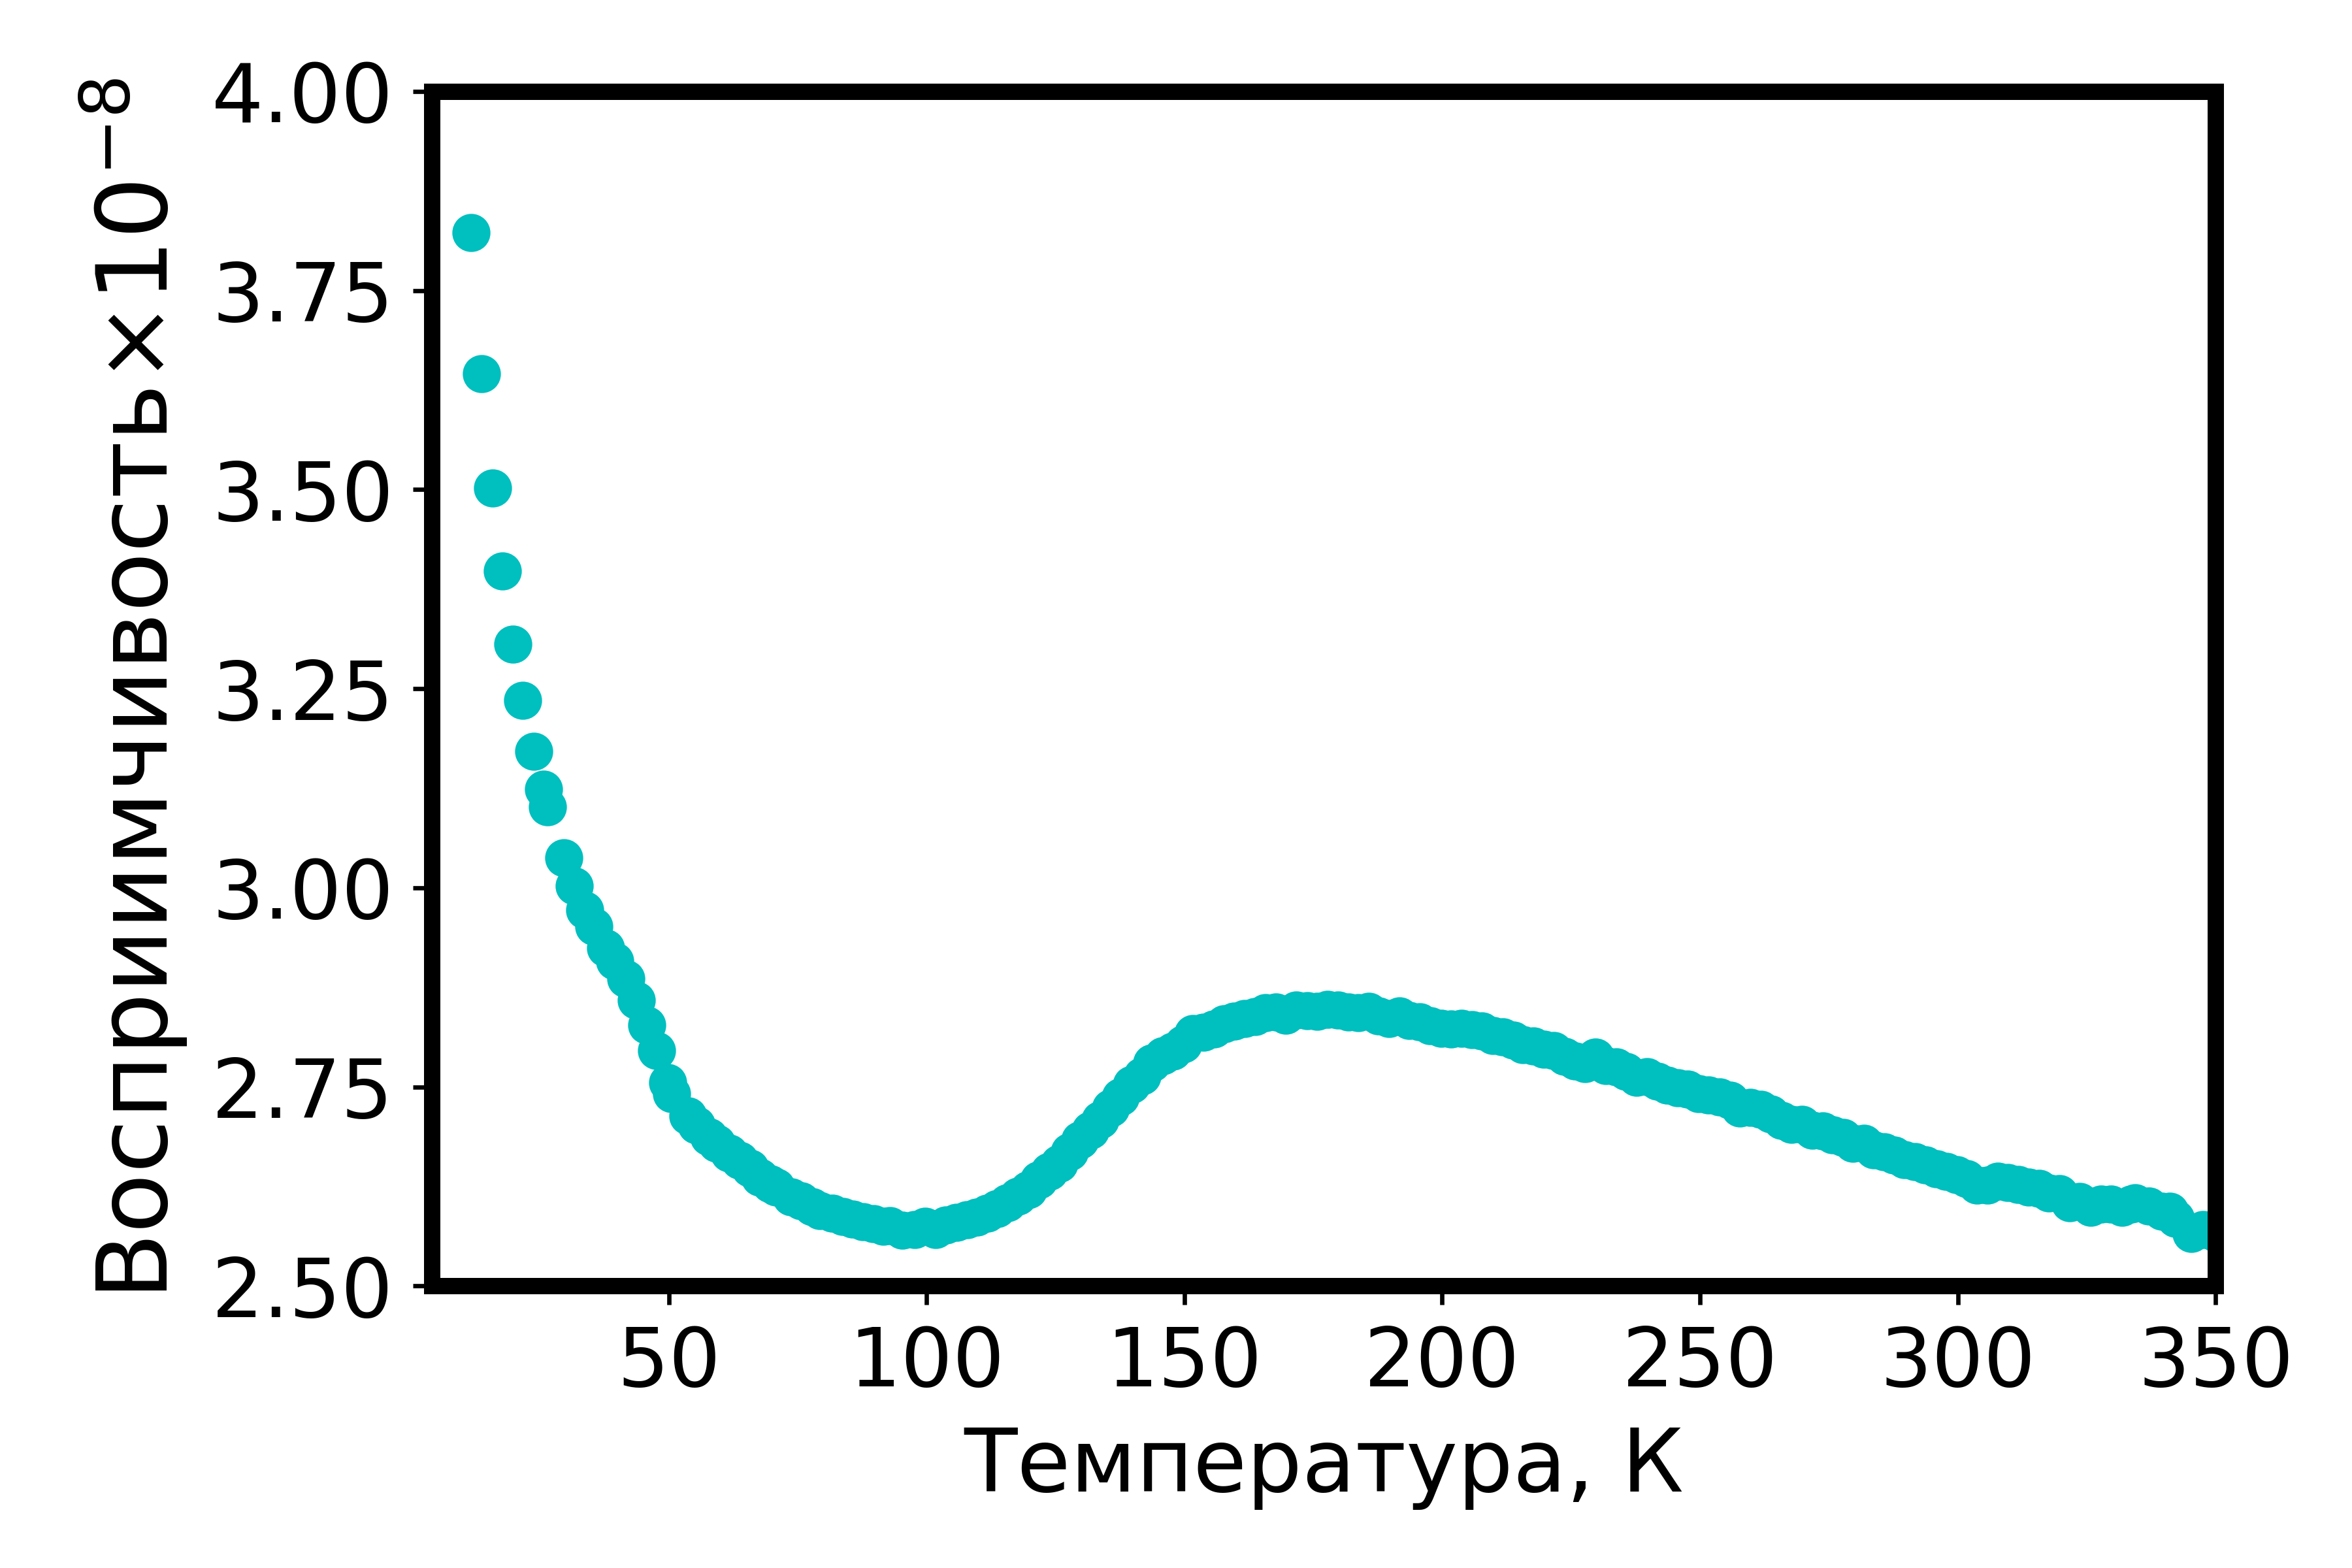
\includegraphics[width=0.9\linewidth]{sus_exp_Cu_As_S} \\ а)
  \end{minipage}
  \hfill
  \begin{minipage}[ht]{0.5\linewidth}\centering
    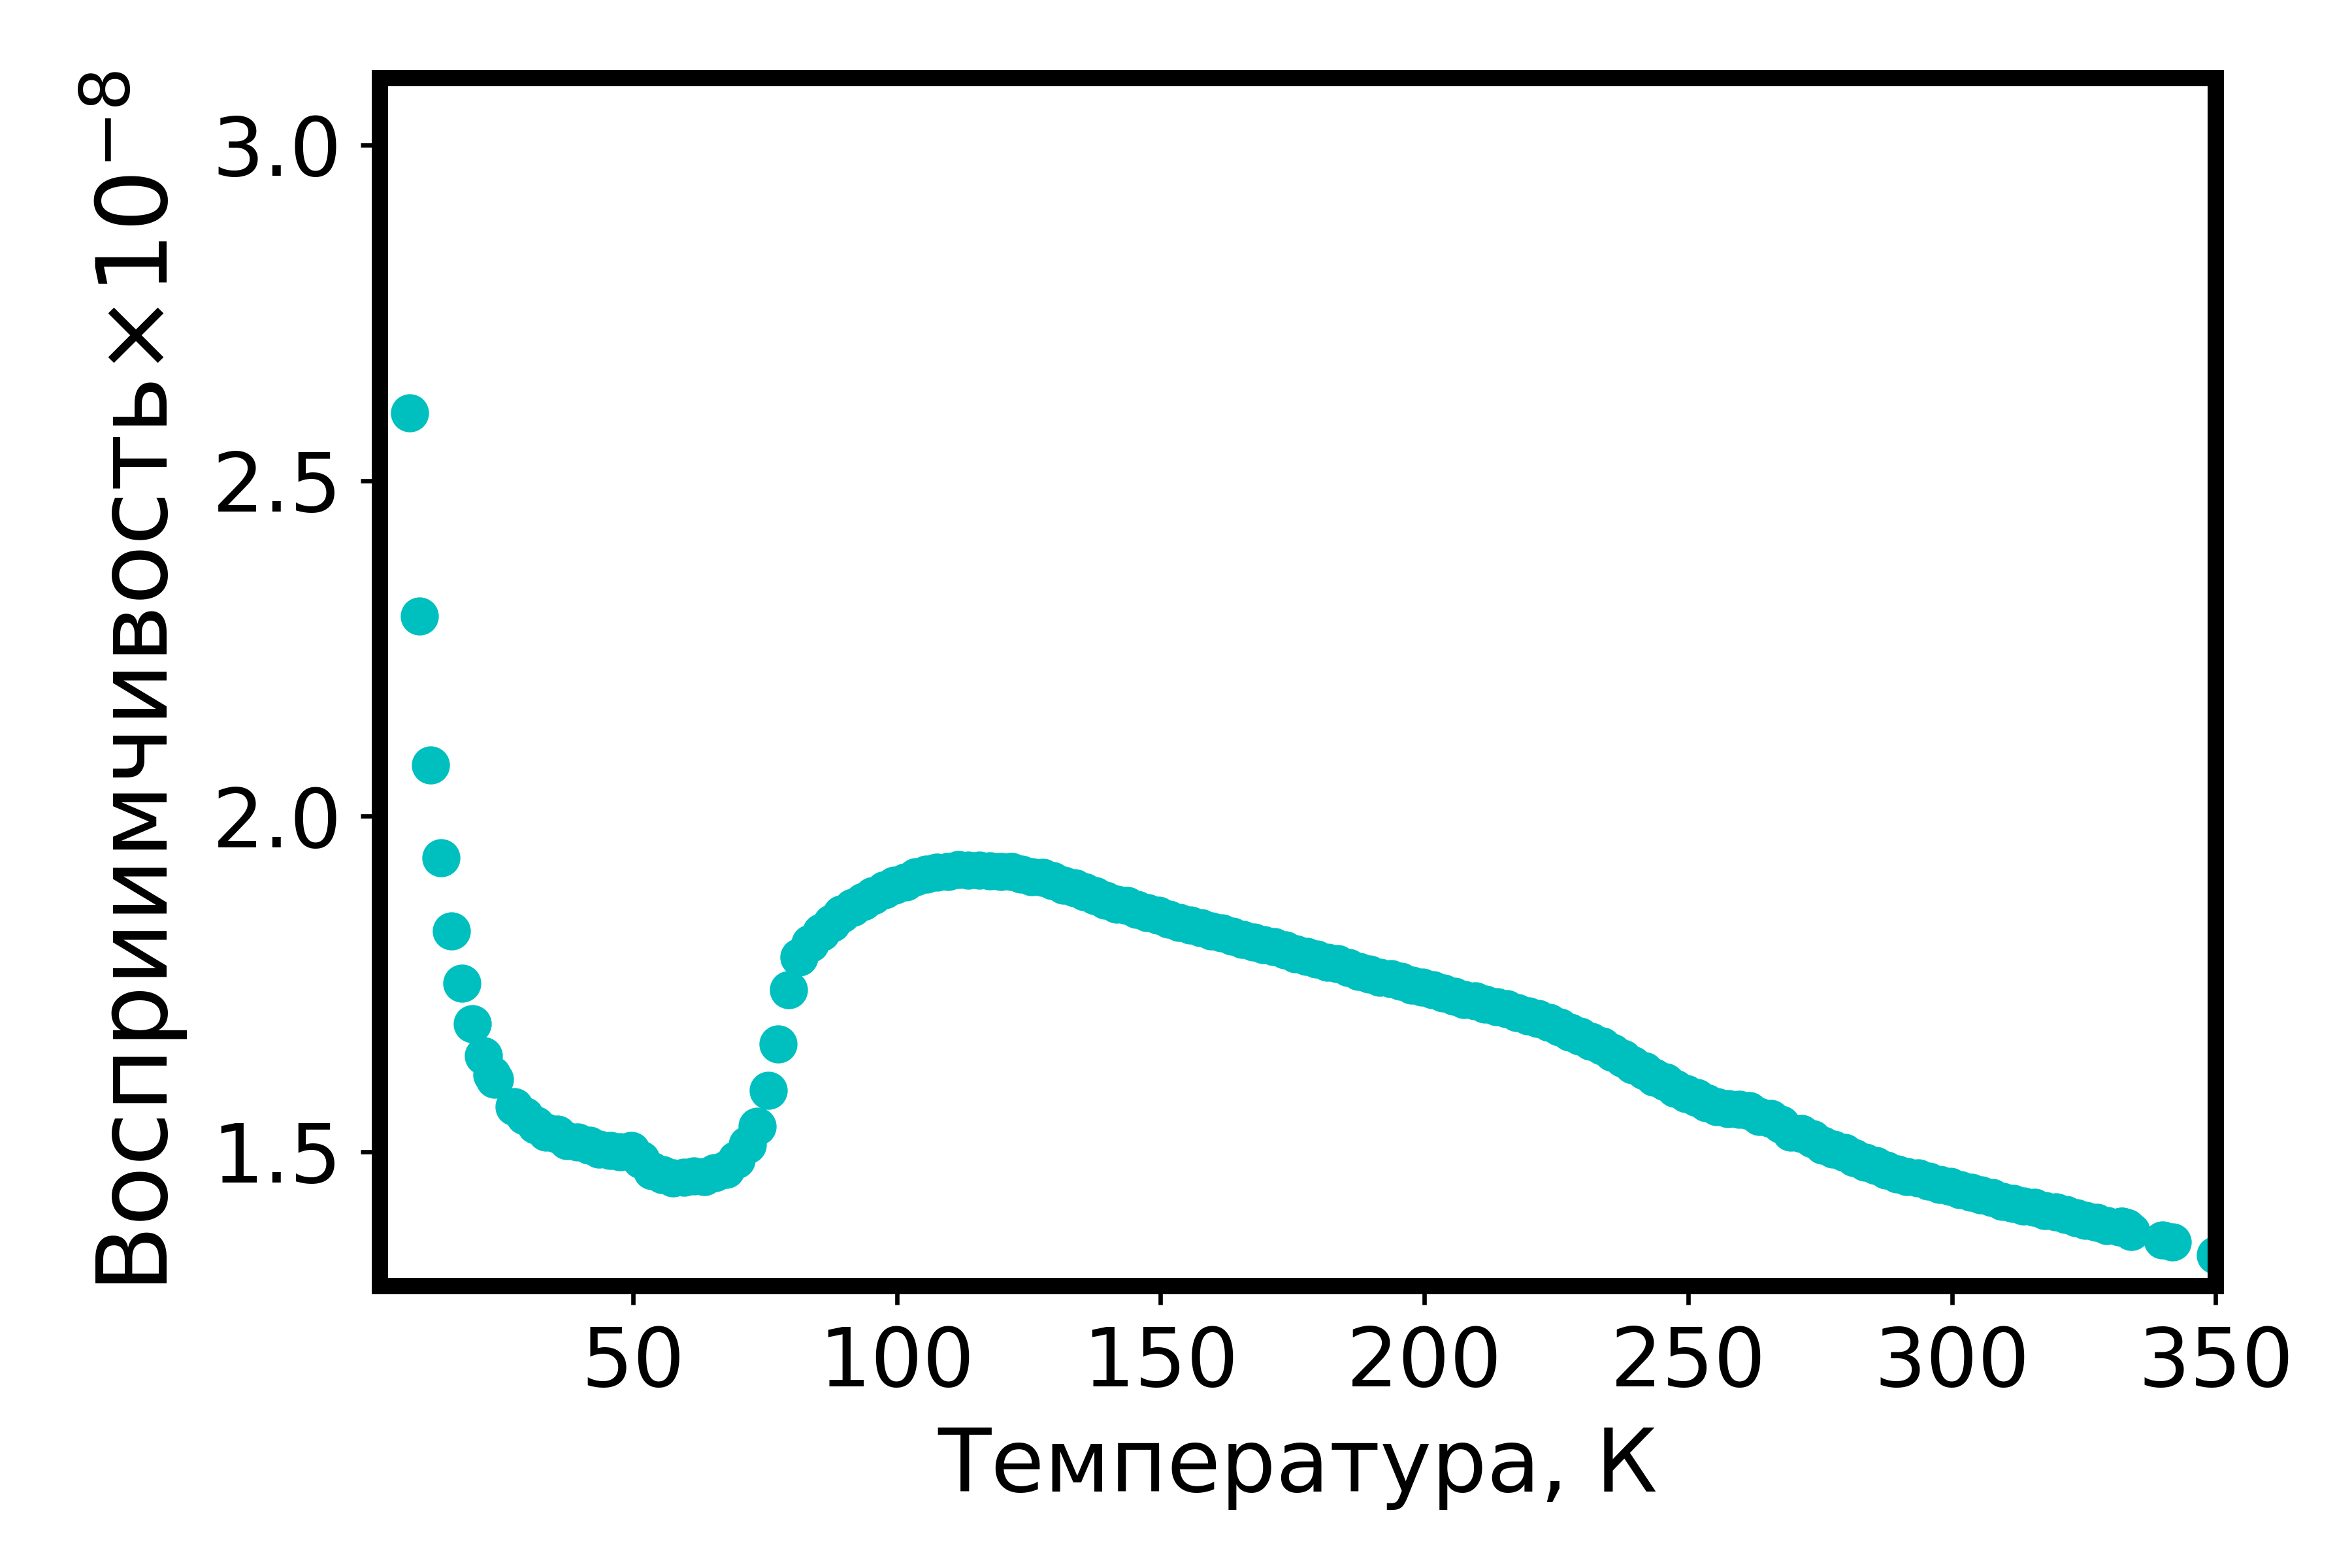
\includegraphics[width=0.9\linewidth]{sus_exp_Cu_Sb_S} \\ б)
  \end{minipage}
\vfill
  \begin{minipage}[ht]{0.5\linewidth}\centering
    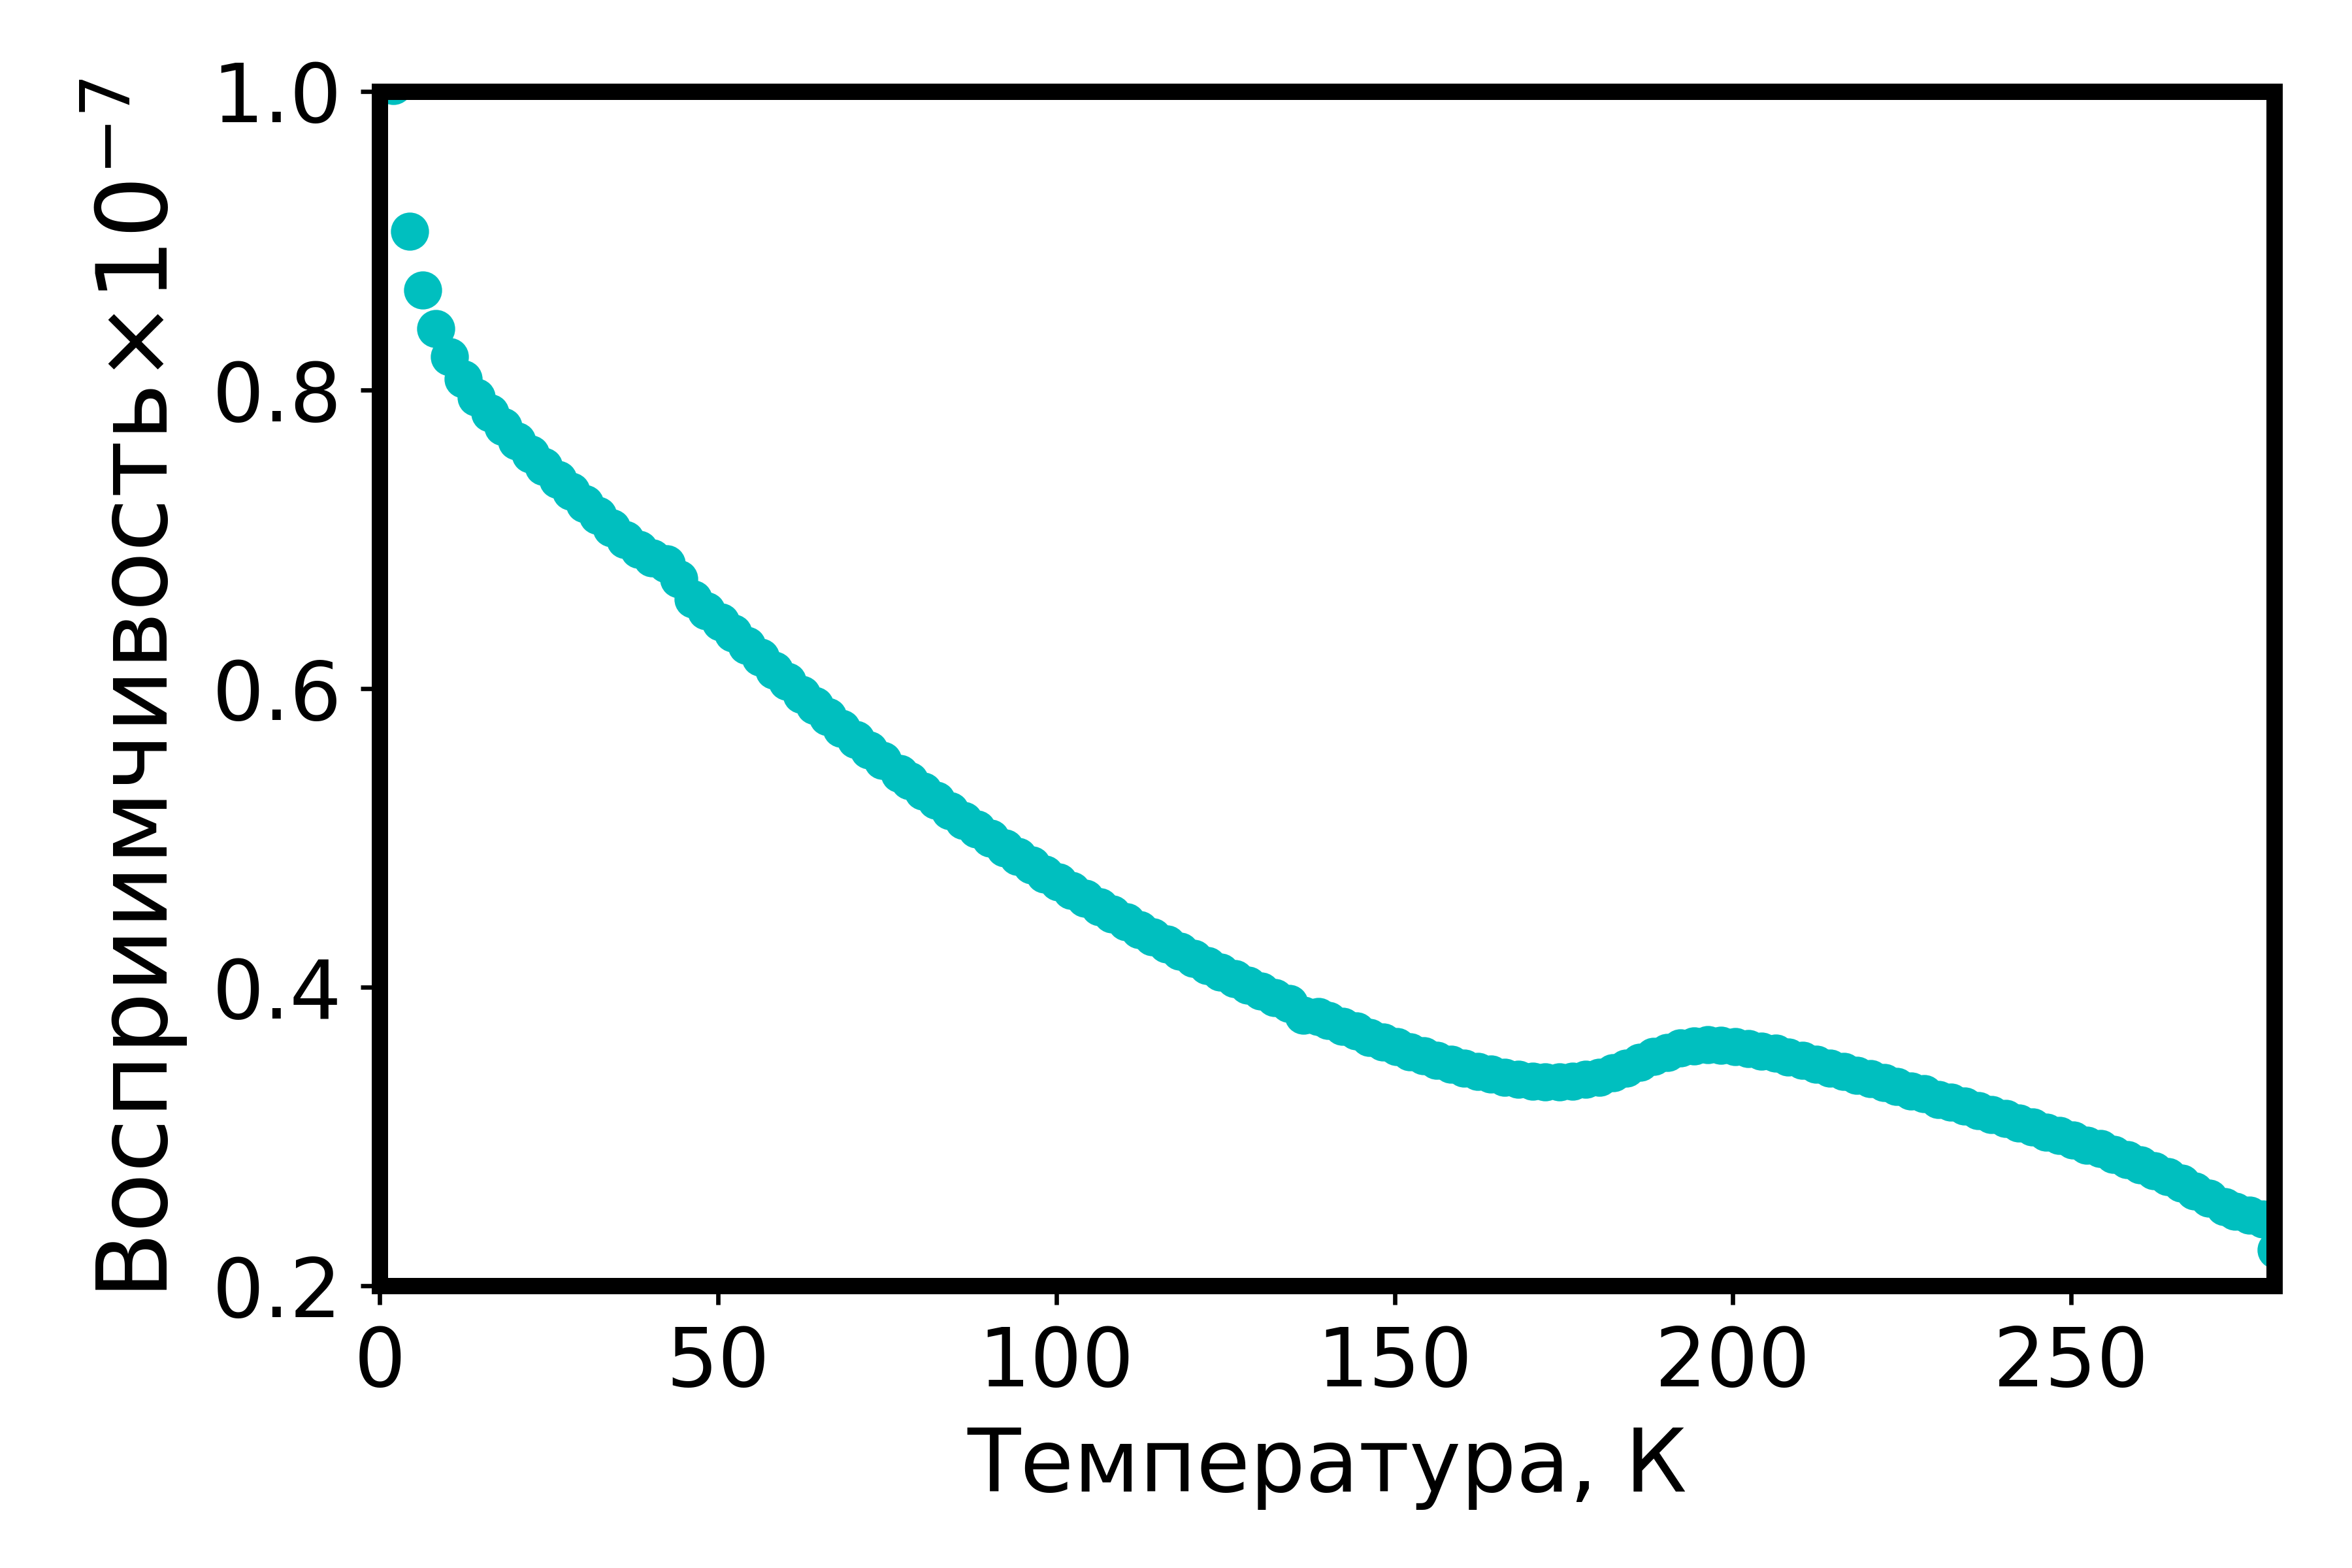
\includegraphics[width=0.9\linewidth]{sus_exp_Cu_As_Se} \\ в)
  \end{minipage}
  \hfill
  \begin{minipage}[ht]{0.5\linewidth}\centering
    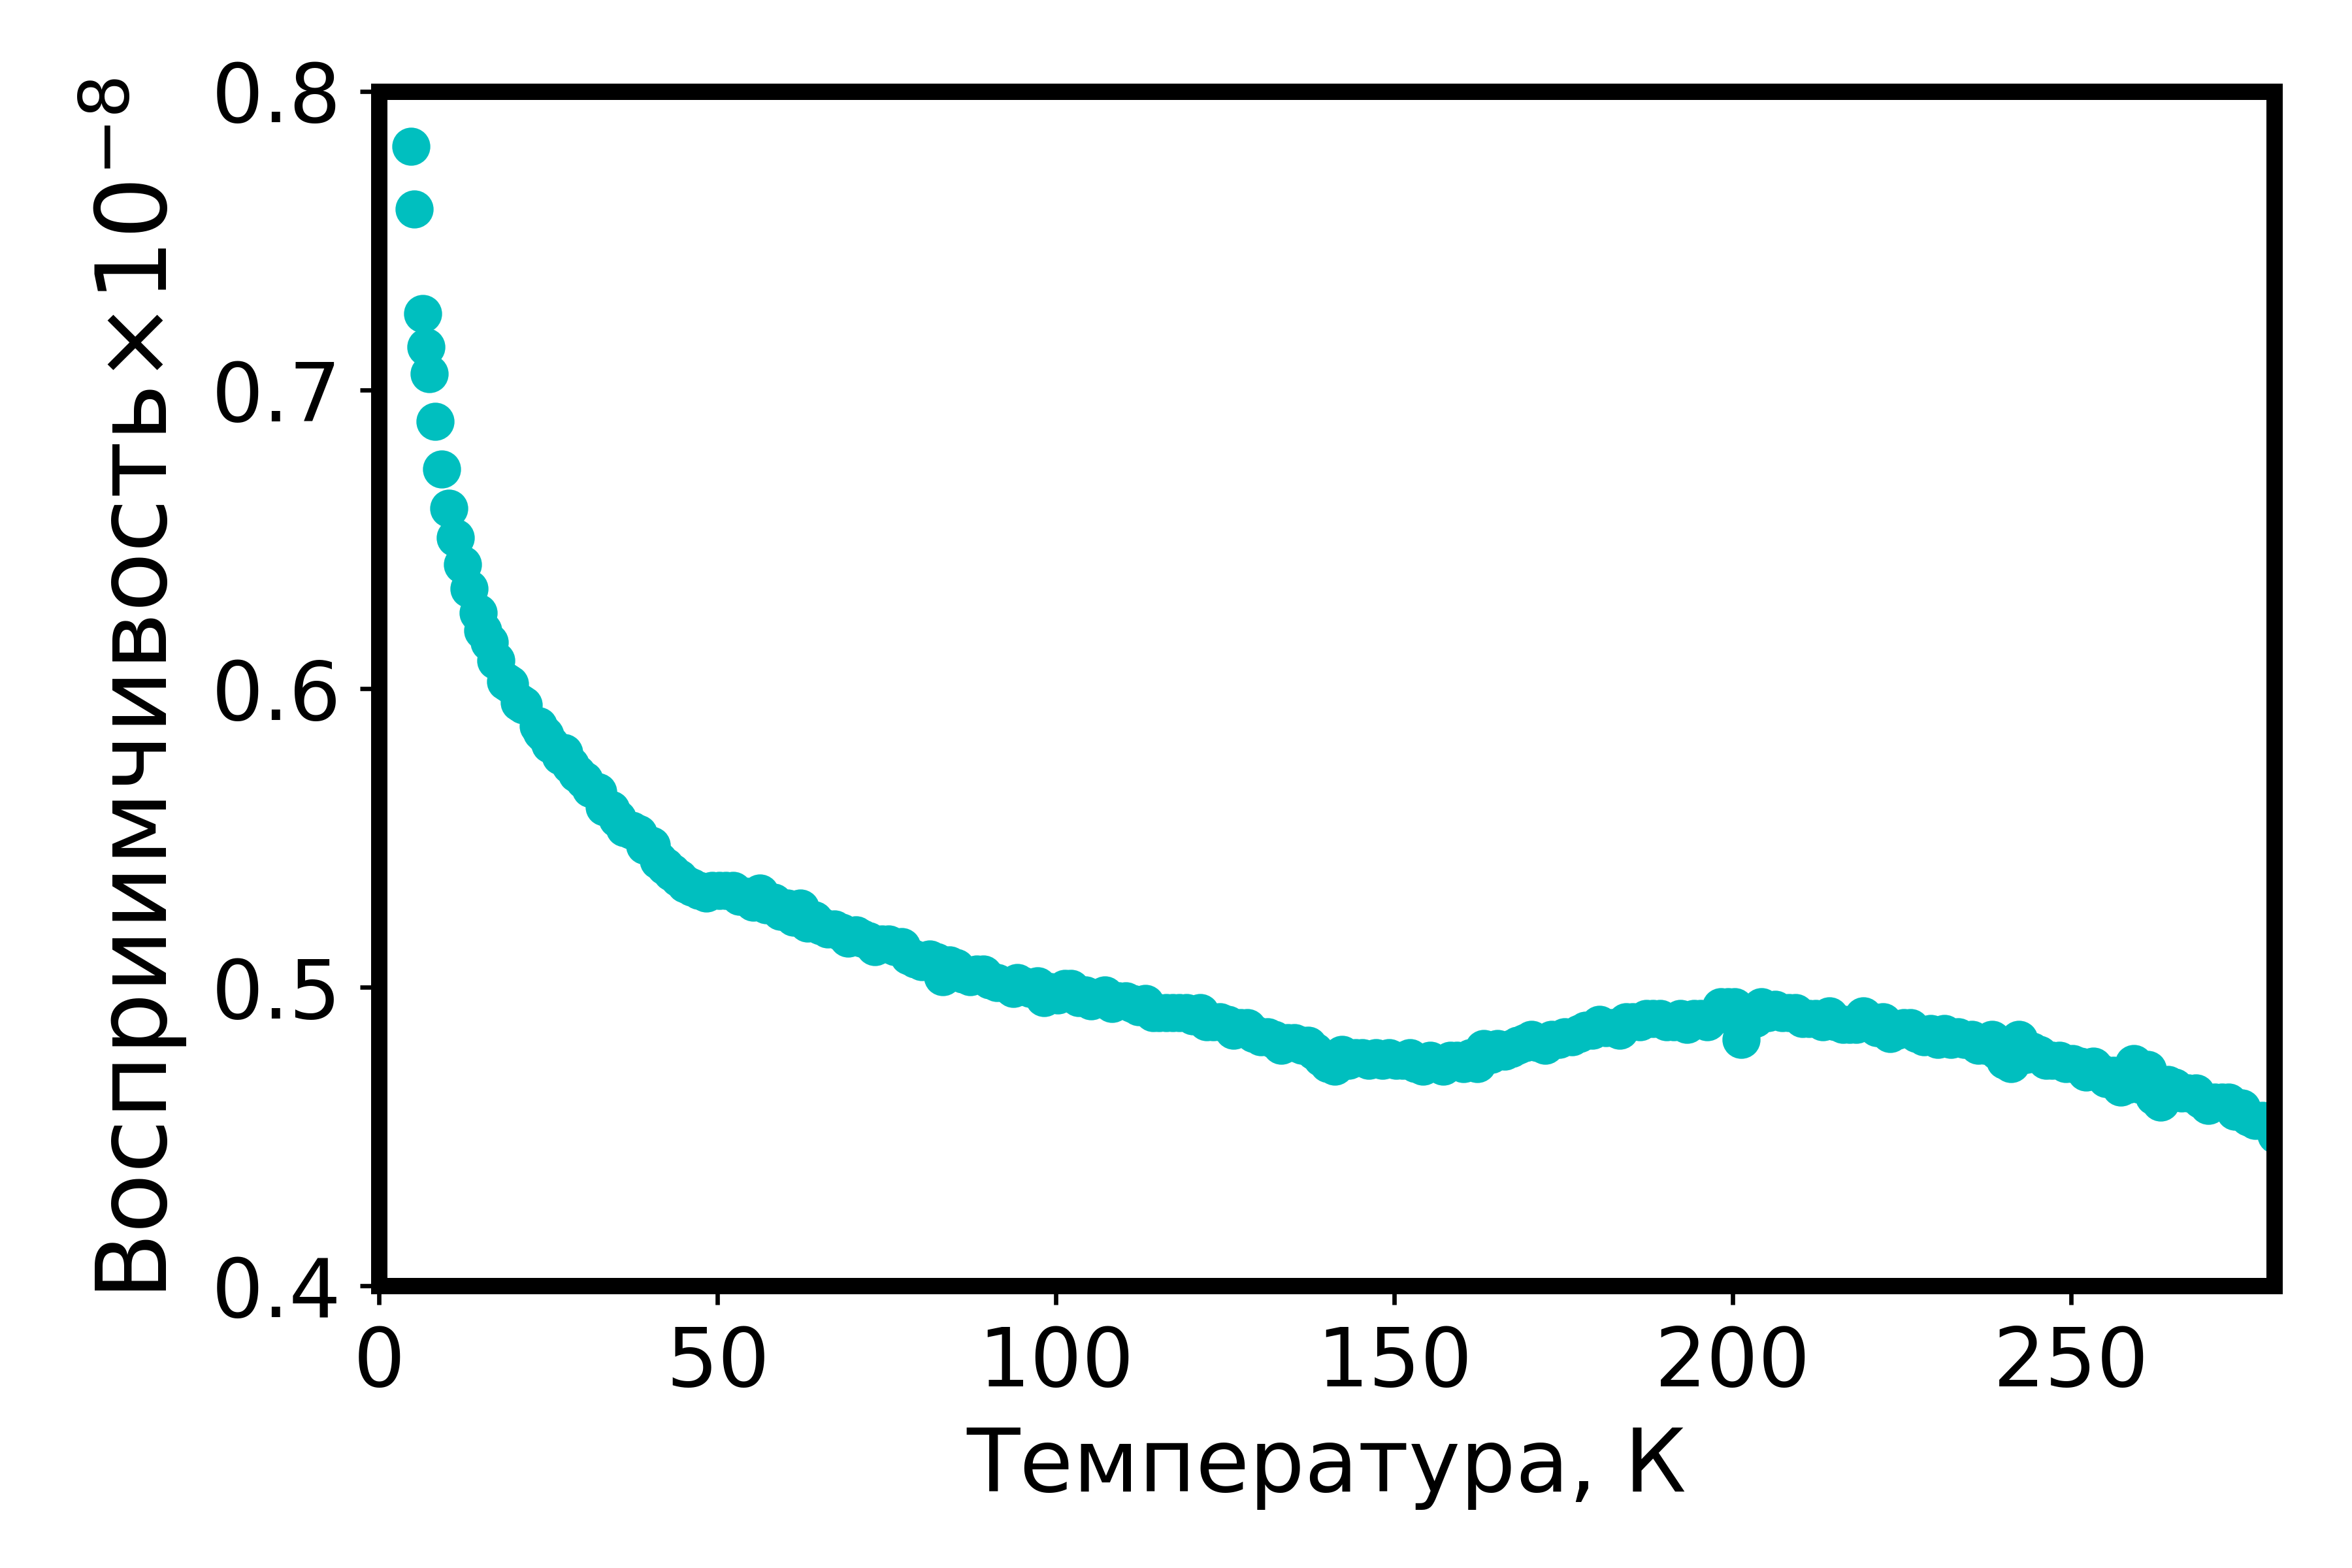
\includegraphics[width=0.9\linewidth]{sus_exp_Cu_Sb_Se} \\ г)
  \end{minipage}

      \caption[Графики температурных зависимостей магнитной восприимчивости для соединений Cu\textsubscript{12}As\textsubscript{4}S\textsubscript{13} (а), Cu\textsubscript{12}Sb\textsubscript{4}S\textsubscript{13} (б), Cu\textsubscript{3}AsSe\textsubscript{3} (в) и Cu\textsubscript{3}SbSe\textsubscript{3} (г)]{Графики температурных зависимостей магнитной восприимчивости для соединений Cu\textsubscript{12}As\textsubscript{4}S\textsubscript{13} (а), Cu\textsubscript{12}Sb\textsubscript{4}S\textsubscript{13} (б), Cu\textsubscript{3}AsSe\textsubscript{3} (в) и Cu\textsubscript{3}SbSe\textsubscript{3} (г)}
    \label{img:figure3}
\end{figure}

Температурные зависимости магнитной восприимчивости для каждого
 образца были получены в магнитных полях 1, 10, 35 и 70 кЭ (Рис. \ref{img:figure3}).
При любом значении магнитного поля графики зависимости магнитной восприимчивости
 имеют одинаковые характерные особенности для всех исследованных соединений.
 Также зависимости магнитной восприимчивости для монокристаллического и
 поликристаллических образцов соединения Cu\textsubscript{12}As\textsubscript{4}S\textsubscript{13} не отличаются.
Все зависимости магнитной восприимчивости приведены с вычетом диамагнитного вклада.
%Полученные зависимости обладают формой, характерной для парамагнетиков с существенными отклонениями от парамагнитного хода.
На графиках температурных зависимостей магнитной восприимчивости для соединений Cu\textsubscript{12}As\textsubscript{4}S\textsubscript{13} и Cu\textsubscript{12}Sb\textsubscript{4}S\textsubscript{13}  наблюдаются отклонения от монотонного парамагнитного хода при температурах T$\approx$124 К и T$\approx$84 К соответственно, и для Cu\textsubscript{3}AsSe\textsubscript{3} и Cu\textsubscript{3}SbSe\textsubscript{3}~"---  T$\approx$170"--~270 К и T$\approx$170"--~300~К соответственно.






%На рисунке~\ref{img:xray} представлены величина заселенности позиций атома Cu2 и изменение значения коэфициента атомарного смещения для позиции атома S2 в диапазоне температур от 85 до 293~К. Аномальное изменение значения коэфициента атомарного смещения для позиции атома S2 показывает наличие фазового перехода второго рода в диапазоне от 115 до 180 К.

%\begin{figure}[ht]
%  \begin{minipage}[ht]{0.5\linewidth}\centering
%    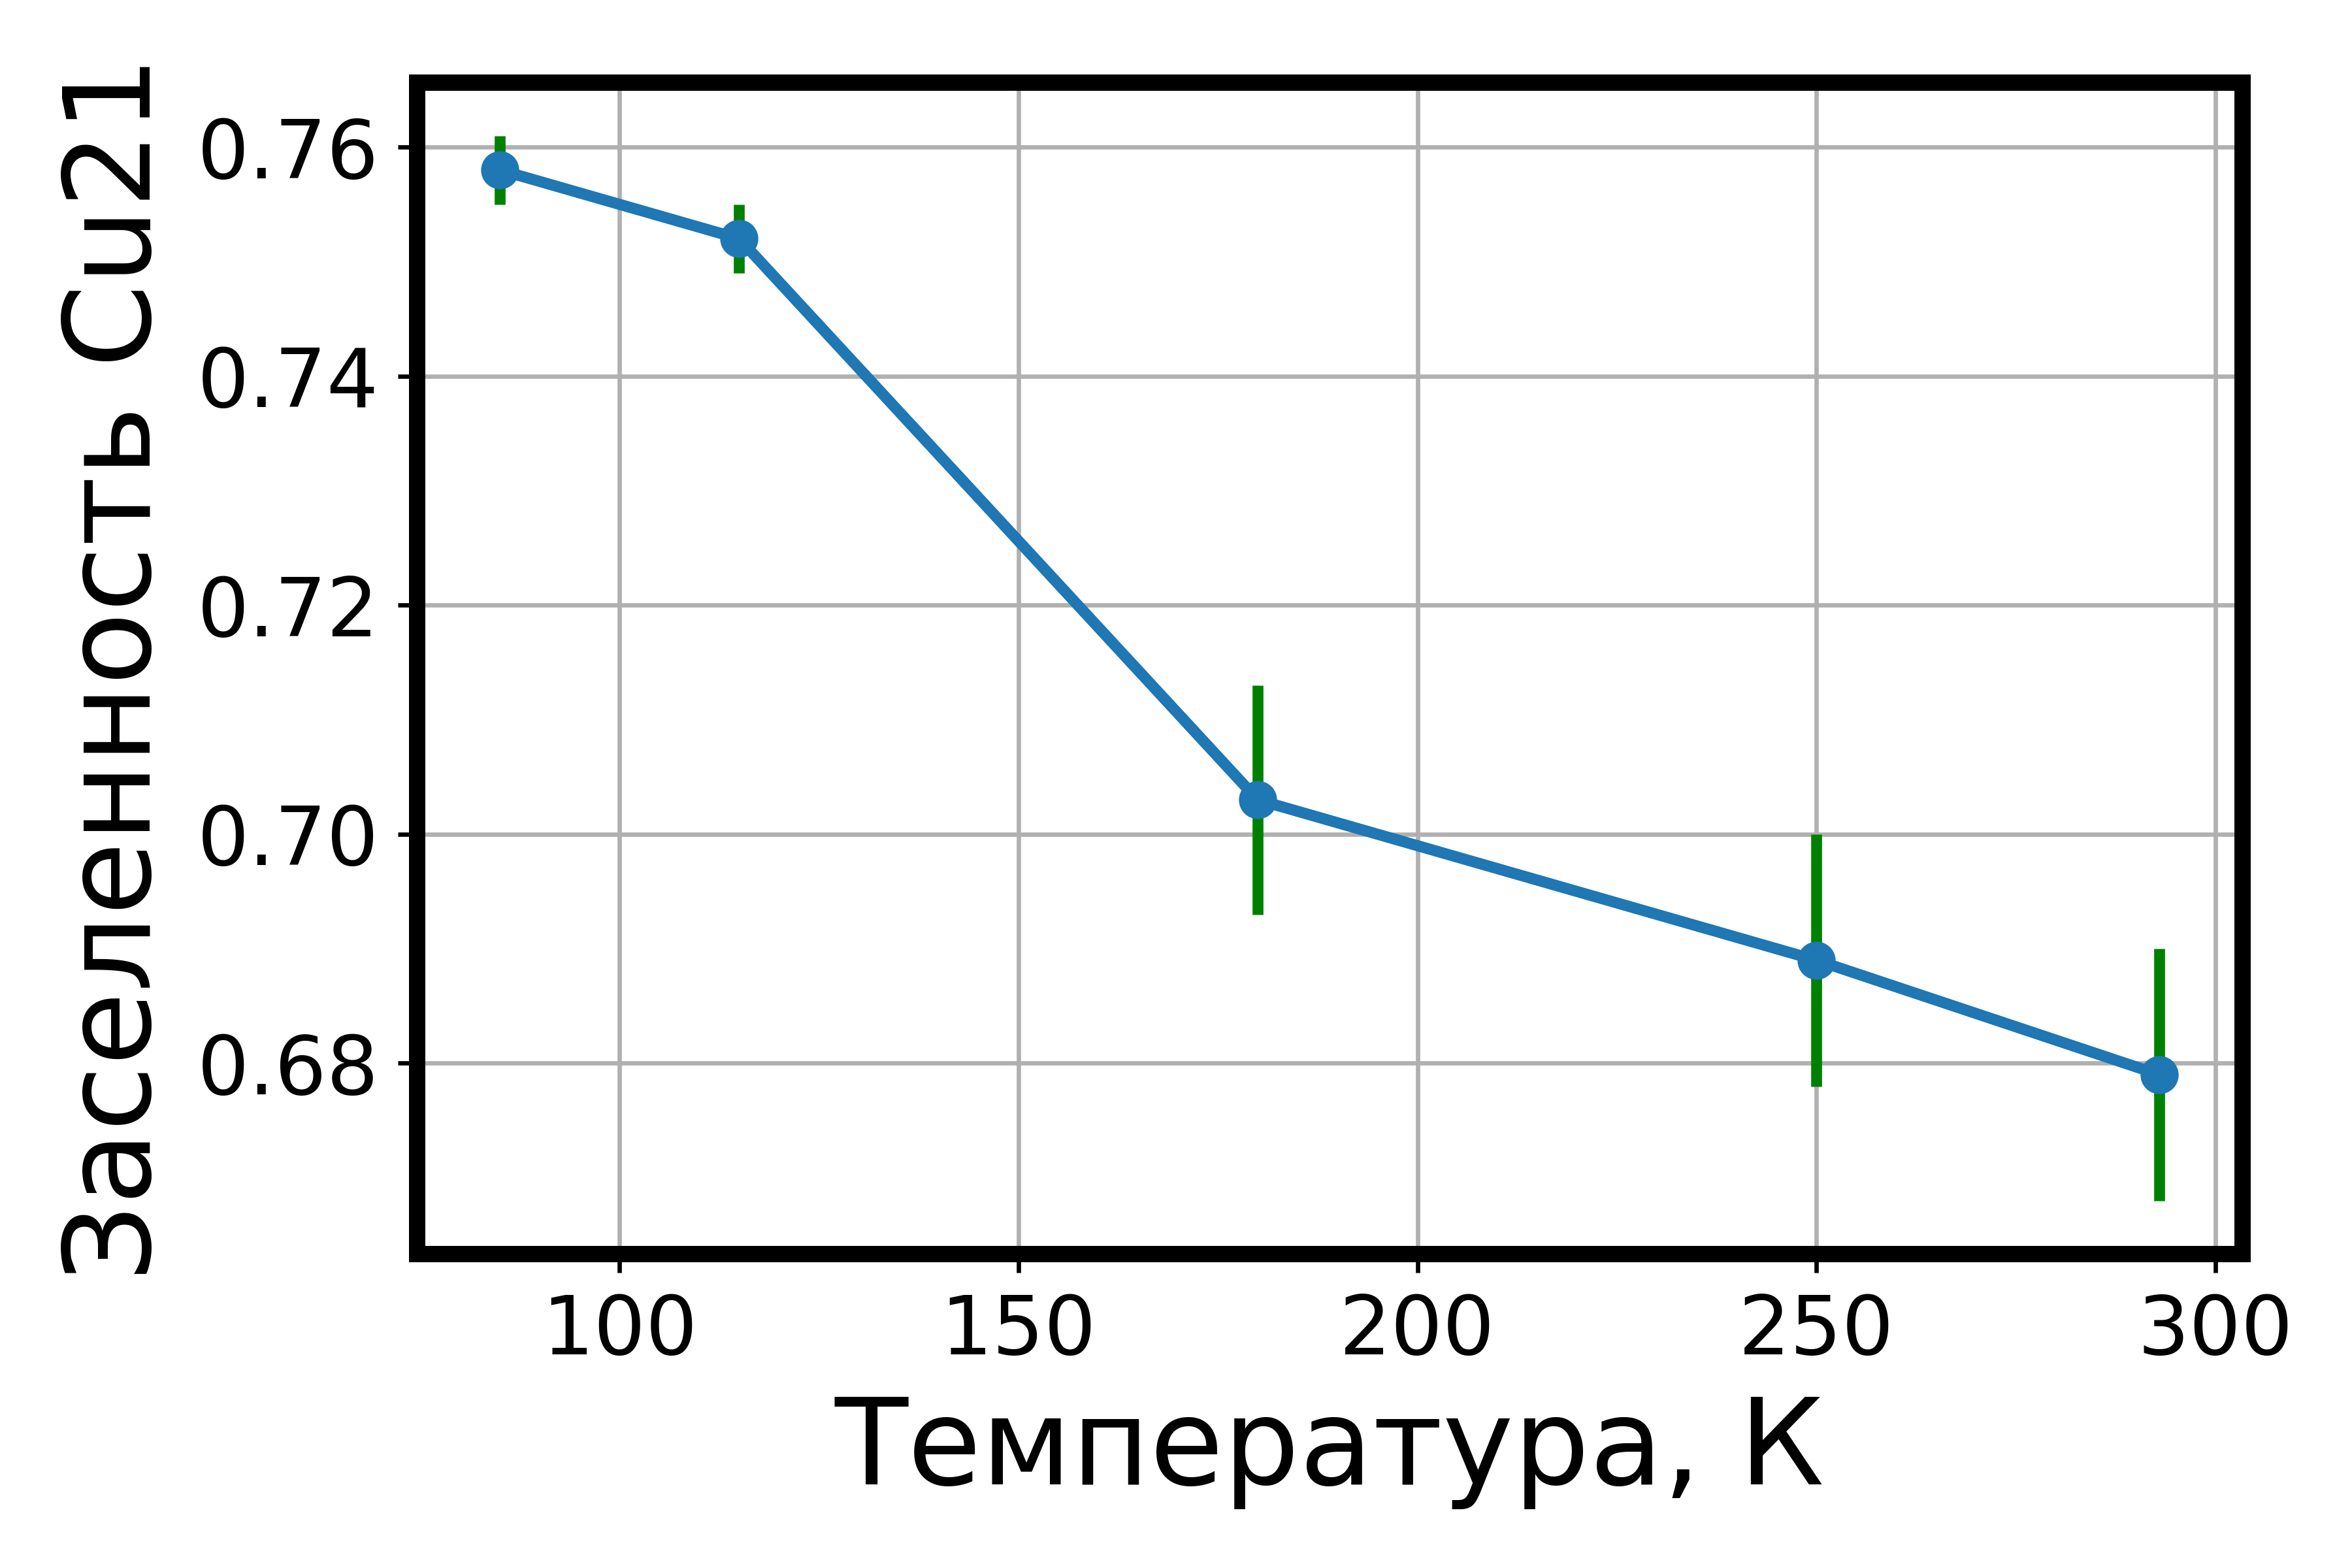
\includegraphics[width=0.9\linewidth]{structure_occCu2} \\ а)
%  \end{minipage}
 % \hfill
 % \begin{minipage}[ht]{0.5\linewidth}\centering
 %   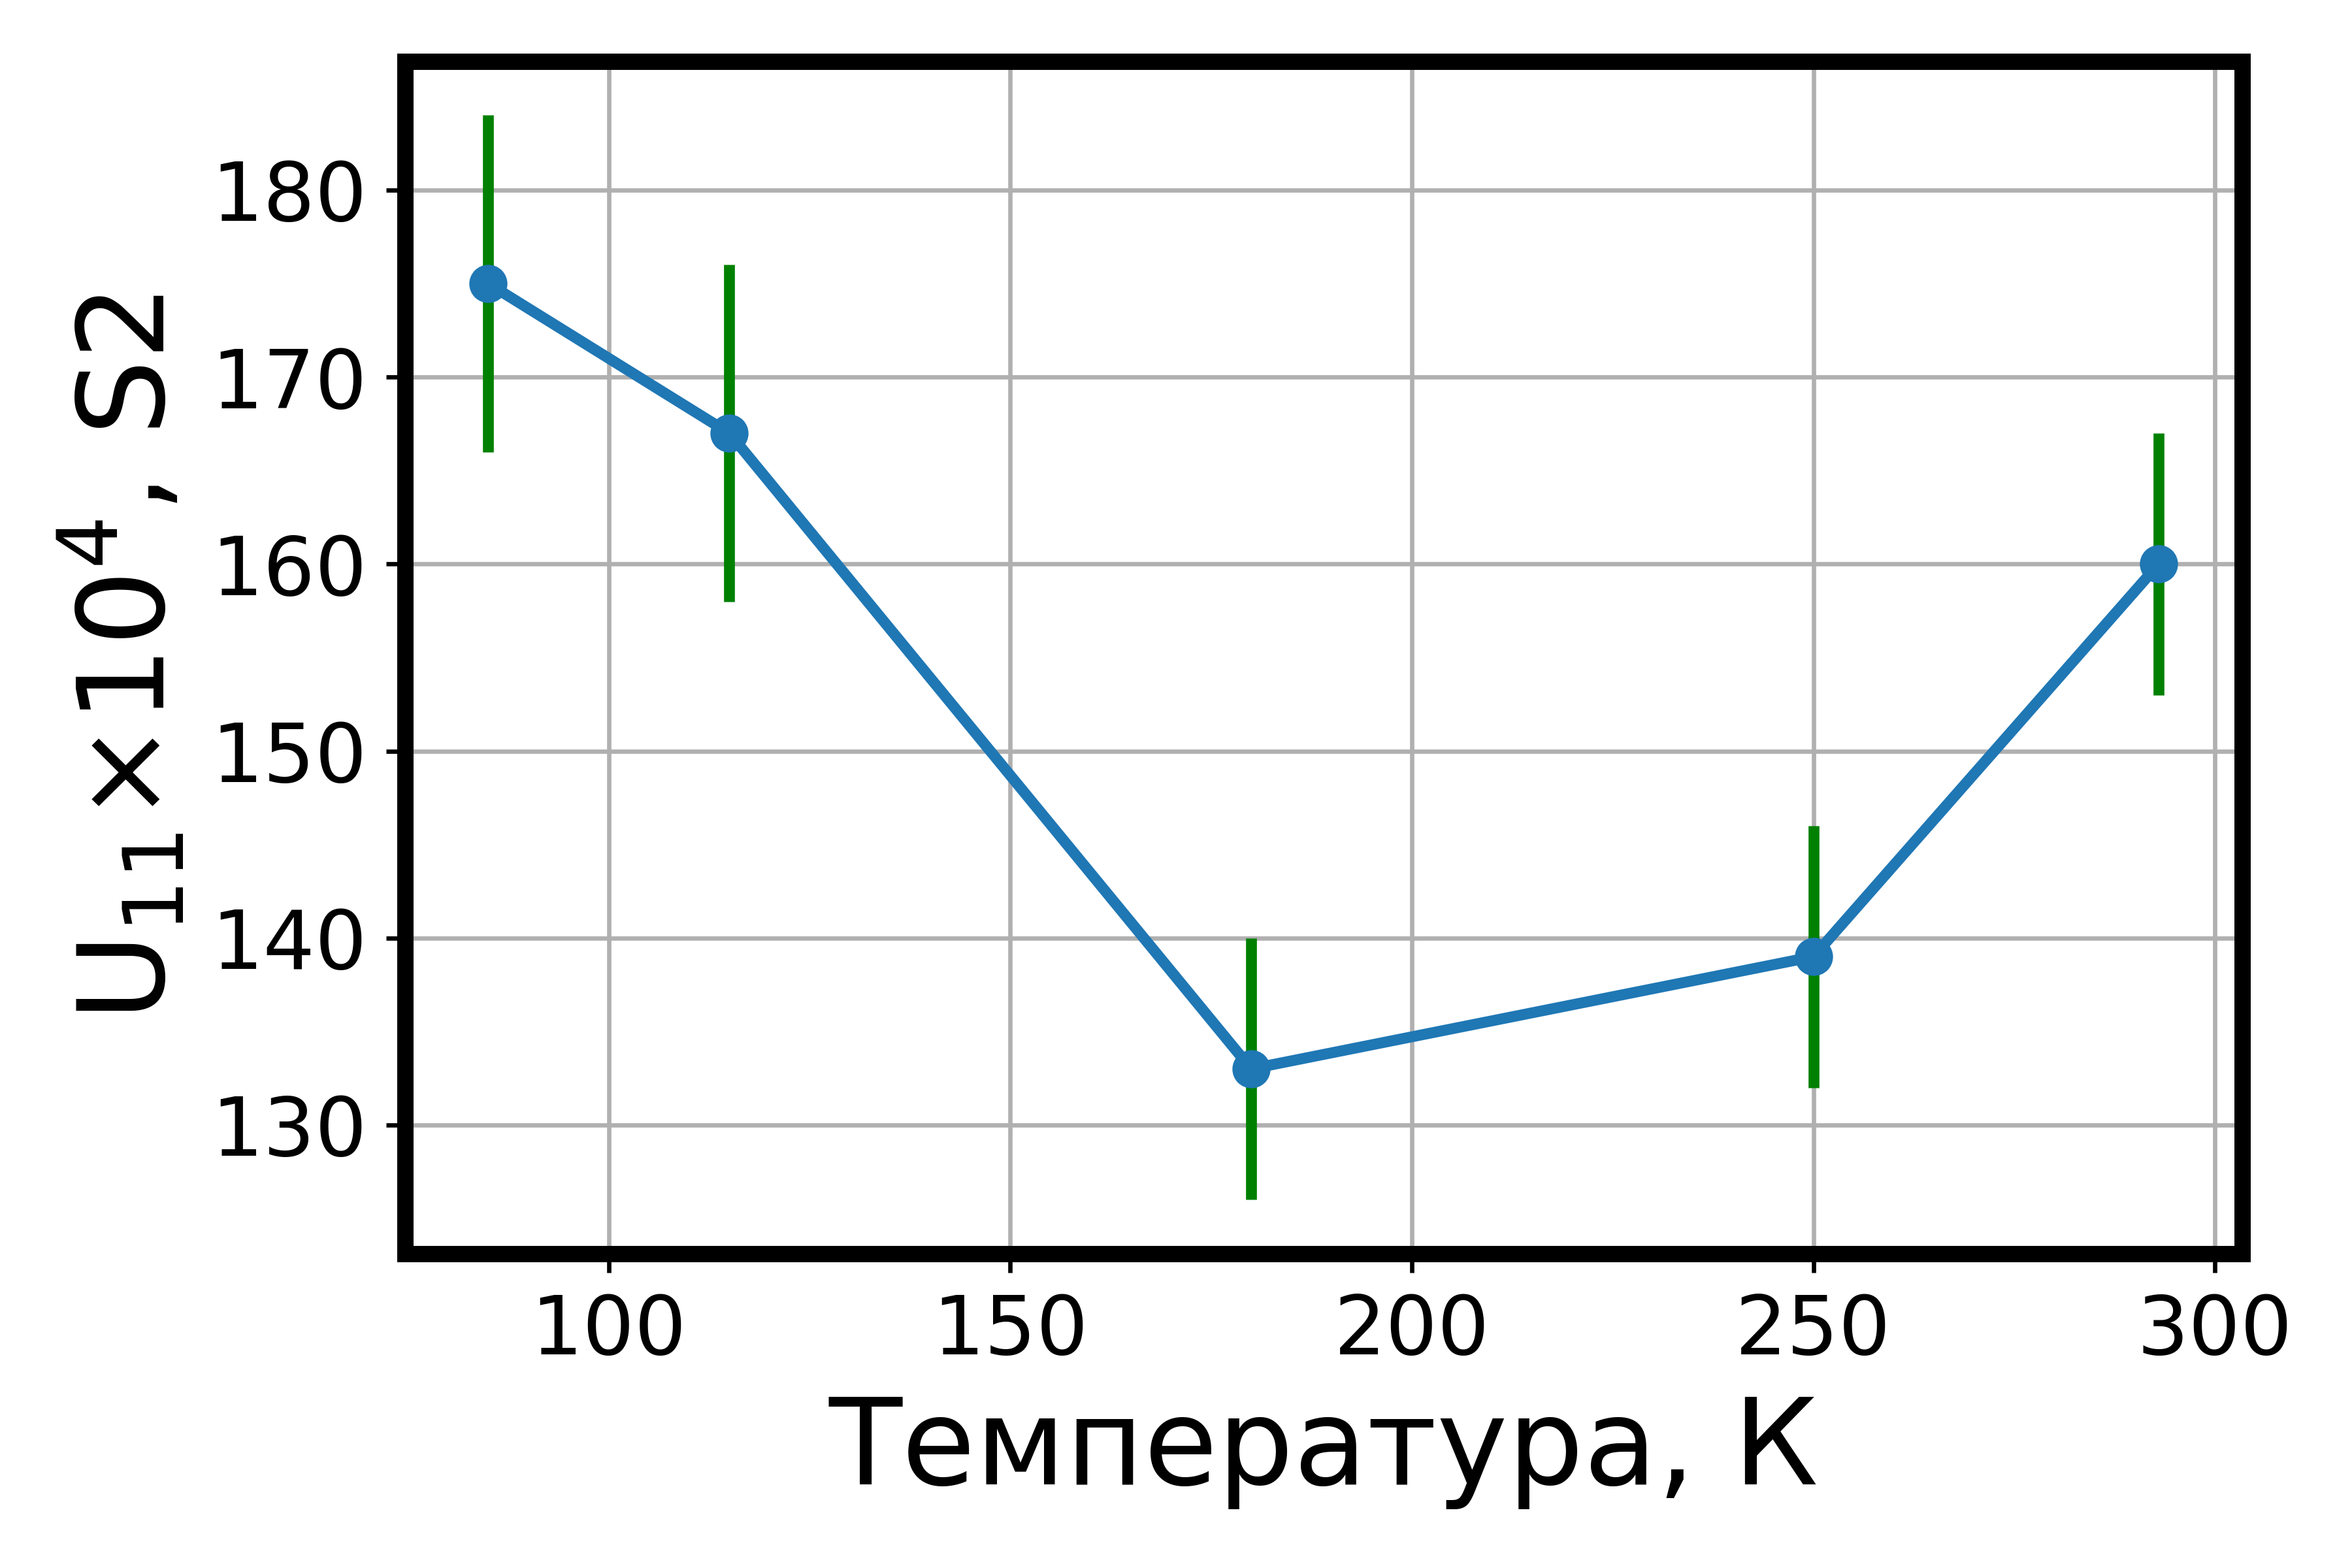
\includegraphics[width=0.9\linewidth]{structure_Ueq} \\ б)
%  \end{minipage}

%      \caption[Значение заселенности позиции атома Cu2 (а) и изменение значения коэффициента атомарного смещения для позиции атома S2 (б) в диапазоне температур от 85 до 293~К синтетического теннантита Cu\textsubscript{12}As\textsubscript{4}S\textsubscript{13}]{Значение заселенности позиции атома Cu2 (а) и изменение значения коэффициента атомарного смещения для позиции атома S2 (б) в диапазоне температур от 85 до 293~К синтетического теннантита Cu\textsubscript{12}As\textsubscript{4}S\textsubscript{13}}
 %   \label{img:xray}
%\end{figure}



Экспериментальная и расчётная зависимости теплоёмкости (Рис.~\ref{img:figure4}) от температуры для синтетического теннантита Сu\textsubscript{12}As\textsubscript{4}S\textsubscript{13} и  синтетического мгриита Cu\textsubscript{3}AsSe\textsubscript{3} удовлетворительно совпадают.
По-видимому, эти моды возникают ввиду ассиметричной связи в As(CuS\textsubscript{3})As, как показывает рентгеноструктурный анализ, в структуре теннантита и, аналогично, в синтетическом мгриите. Такие моды уменьшают решеточную теплопроводность и, как следствие, улучшают термоэлектрические свойства.

Анализ влияния изовалентного замещения на температурные зависимости магнитной восприимчивости (Рис.~\ref{img:figure3}) и на спектры комбинационного рассеяния (Рис.~\ref{img:figure_raman}) показывает, что изменение локального окружения меди приводит к изменению температур магнитных изменений и энергий низкоэнергетических фононных мод. В случае синтетического теннантита Cu\textsubscript{12}As\textsubscript{4}S\textsubscript{13} получено, что АФМ упорядочение энергетически более выгодно, чем другие типы состояний.

В \underline{\textbf{заключении}} приведены основные результаты работы и выводы, которые заключаются в следующем:
%% Согласно ГОСТ Р 7.0.11-2011:
%% 5.3.3 В заключении диссертации излагают итоги выполненного исследования, рекомендации, перспективы дальнейшей разработки темы.
%% 9.2.3 В заключении автореферата диссертации излагают итоги данного исследования, рекомендации и перспективы дальнейшей разработки темы.
\begin{enumerate}
						\item На основе анализа экспериментальных данных, полученных в рентгеноструктурных температурных экспериментах, элекронной микроскопии и на основе результатов квантомеханического моделирования, установлено, что
						лавесовский полиэдр сформирован шестью атомами меди, которые лежат в неэквивалентных позициях Cu2 и Cu21, а на структурную формулу синтетического теннантита Сu\textsubscript{12}As\textsubscript{4}S\textsubscript{13} приходится 12 атомов меди.
						\item Через сравнение данных расчётной  и  экспериментальной теплоёмкостей, полученной сканирующей дифференциальной калориметрией и спектроскопии комбинационного рассеяния света при комнатной температуре, показано влияние ассиметричной связи As(CuS\textsubscript{3})As, возникающей ввиду наличия неэквивалентных позициий Cu2 и Cu21, на размягчение фононных мод в структуре синтетического теннантита Сu\textsubscript{12}As\textsubscript{4}S\textsubscript{13}.
						\item Методами рентгеноструктурного анализа, сканирующей дифференциальной калориметрии, магнитометрии и первопринципных расчётов обнаружен фазовый переход второго рода в синтетическом теннантите Сu\textsubscript{12}As\textsubscript{4}S\textsubscript{13} при температуре 124 К.
						\item Методами сканирующей дифференциальной калориметрии, магнитометрии и спектроскопии комбинационного рассеяния света выявлены  низкоэнергетические фононные моды (ввиду  ассиметричной связи в (As,Sb)(Cu(S, Se)\textsubscript{3})(As,Sb)) в  соединениях из группы тетраэдритов-теннантитов. Найденные значения энергий фононных мод лежат в диапазоне от 5 до 40~мэВ.
						\item На основе результатов работы и опубликованных литературных данных рассмотрено влияние изовалентного замещения в Cu--(As,Sb)--S на значения температур фазовых переходов второго рода.

\end{enumerate}



%\newpage
%При использовании пакета \verb!biblatex! список публикаций автора по теме
%диссертации формируется в разделе <<\publications>>\ файла
%\verb!../common/characteristic.tex!  при помощи команды \verb!\nocite!

\ifthenelse{\equal{\thebibliosel}{0}}{% Встроенная реализация с загрузкой файла через движок bibtex8
  \renewcommand{\refname}{\large \authorbibtitle}
  \nocite{*}
  \insertbiblioauthor                          % Подключаем Bib-базы
  %\insertbiblioother   % !!! bibtex не умеет работать с несколькими библиографиями !!!
}{% Реализация пакетом biblatex через движок biber
  \insertbiblioauthor                          % Подключаем Bib-базы
  \insertbiblioother
}
